\documentclass{article}

% NeurIPS 2026 style --- swap \usepackage{iclr2024_conference} for
% \usepackage[preprint]{neurips_2026} once the official .sty is released.
\usepackage{iclr2024_conference}

% Core packages
\usepackage{amsmath,amssymb,amsfonts}
\usepackage{graphicx}
\usepackage{booktabs}
\usepackage{url}
\usepackage{xcolor}
\usepackage{algorithm}
\usepackage{algpseudocode}
\usepackage{subcaption}
\usepackage{multirow}
\usepackage{array}
\usepackage{pifont}       % \ding{51} checkmark, \ding{55} cross
\usepackage[utf8]{inputenc}
\usepackage[T1]{fontenc}
\usepackage{hyperref}

\hypersetup{
    colorlinks=true,
    linkcolor=blue!70!black,
    citecolor=blue!70!black,
    urlcolor=blue!70!black,
}

% Natbib --- author-year citations
\usepackage{natbib}
\bibliographystyle{iclr2024_conference}
\setcitestyle{authoryear,open={(},close={)}}

% -----------------------------------------------------------------------
\title{\textbf{TEL-OS: Inference-Only Representation Governance Eliminates Adversarial Jailbreak Optimization}}

\author{Josue Gutierrez Alvarez Tostado \\
\texttt{\href{https://x.com/josuetoz}{x.com/josuetoz}}}

\iclrfinalcopy  % Activates NeurIPS 2026 preprint header

\begin{document}
\maketitle

% -----------------------------------------------------------------------
\begin{abstract}
Optimized adversarial attacks---genetic suffix optimization, semantic inversion,
stacked identity-hijacking, and autonomous multi-turn LRM agents---reduce the
safety of RLHF-aligned LLMs to near zero: frontier models suffer 97.14\% Attack
Success Rate (ASR) against LRM autonomous agents \citep{hagendorff2026lrm}, and
existing inference-time defenses fail to close this gap without weight modification
or prohibitive overhead.
We present \textbf{TEL-OS v3.0}, an inference-only governance framework that closes
this gap via \textit{adaptive per-layer refusal steering}: per-layer refusal
direction extraction (\textsc{OBLITERATUS}), dual-layer OR-logic detection at
architecturally consistent depths (${{\sim}}40\%$ and ${{\sim}}70\%$), and
urgency-scaled geometry-preserving steering with zero weight modification.

On Llama-3.1-8B-Instruct, TEL-OS achieves \textbf{0.00\% ASR} against every
optimized attack paradigm evaluated:
LRM autonomous multi-turn attacks are blocked across 200 independent trials
(4 frontier attackers: DeepSeek-R1, GPT-4o, Qwen3-235B, Gemini~2.5~Flash),
95\% CI $[0.00\%,\,1.83\%]$, model-as-a-judge evaluation;
AutoDAN-Turbo genetic optimization produces \texttt{best\_loss}$=0.5$ from step~1
with no improvement across 50 behaviors;
FlipAttack semantic inversion \citep{liu2025flipattack} achieves 0.00\% effective ASR;
and stacked 6-component identity-hijacking (GODMODE + Parseltongue + prefill
forcing + $T{=}1.7$) achieves 0.00\% ASR across 52 high-severity behaviors
(95\% CI $[0.00\%,\,6.85\%]$).
TEL-OS also achieves 0.00\% ASR on direct-prompt benchmarks (AdvBench 520,
HarmBench 400), 0.00\% incremental false positive rate (200 MT-Bench prompts),
and 15.2\% throughput reduction ($+4.56$~ms/token on RTX~4090).
Cross-model deployment across five architectures yields 0.00--0.38\% ASR on
AdvBench; HarmBench residuals (up to 7.00\%) require per-corpus vector
re-extraction and are not universally corpus-agnostic out of the box.

These results establish that \textit{adaptive inference-time steering over internal
refusal representations is sufficient to collapse the loss landscape of adaptive
attacks}---including autonomous LRM agents operating with full strategic
freedom---without retraining, weight modification, or accuracy degradation.
The geometry-preserving property of SLERP (Norm Drift $\approx 1.0000$) ensures
steered activations remain on the pretraining manifold; however, it is the
adaptive urgency-scaled intervention---not the specific interpolation operator---
that collapses the adversarial optimization signal.
\end{abstract}

% -----------------------------------------------------------------------
\section{Introduction}
\label{sec:introduction}

Frontier LLMs are near-fully compromised by optimized adversarial attacks:
autonomous multi-turn LRM agents achieve \textbf{97.14\% ASR} on GPT-4o,
Claude~4~Sonnet, and Gemini~2.5~Flash \citep{hagendorff2026lrm};
genetic suffix optimization (AutoDAN-Turbo) reaches \textbf{80--90\% ASR}
\citep{liu2024autodan};
and semantic inversion (FlipAttack) exceeds \textbf{70\% ASR} on frontier models
\citep{liu2025flipattack}.
Modern RLHF-aligned models exhibit only 3--8\% vulnerability to \textit{direct}
prompts---but this provides false assurance.
The operationally relevant threat is \textit{optimized} attack, where undefended
models are near-fully compromised and existing inference-time defenses
consistently fail to close the gap.

Existing defenses face a structural trilemma.
\textit{Weight-based} approaches (RLHF, SFT, abliteration) modify the model
permanently and fail to generalize to novel attack distributions.
\textit{Input-filtering} defenses (SmoothLLM, paraphrase detection) impose
high inference overhead and are bypassable via semantic reframing.
\textit{Representation-based} methods (RepE, Activation Addition) show promise
but rely on \textit{linear} steering that introduces geometric distortion into
the activation space---an underexplored failure mode at non-negligible steering
strengths.

We propose \textbf{TEL-OS v3.0}, an inference-only governance framework that
resolves this trilemma via \textit{adaptive per-layer refusal steering}:
per-layer refusal direction extraction (\textsc{OBLITERATUS}), dual-layer
OR-logic detection at architecturally consistent depths (${{\sim}}40\%$ and
${{\sim}}70\%$), and urgency-scaled steering whose response intensity grows
proportionally with the attack's geometric displacement from the refusal manifold.
This adaptive coupling is the mechanistic source of the \textit{Guillotina
Ge\'om\'{e}trica}: the more effectively an adversarial suffix shifts the activation
away from the refusal direction, the stronger the correction---making the genetic
optimization loss landscape flat from step~1 (Section~\ref{subsec:guillotina}).
For the steering operator we use Spherical Linear Interpolation (SLERP): a
geometry-preserving choice that constrains steered activations to the pretraining
hypersphere (Norm Drift $0.999992 \pm 0.0004$ vs.\ $+22.2\%$ for linear steering),
but equivalent in defense efficacy to linear steering on current benchmarks
(both 0.00\% ASR, XP-36a; see Section~\ref{subsec:slerp_geometry}).

\paragraph{Contributions.}
\begin{itemize}
    \item[\textbf{C1.}] \textbf{TEL-OS v3.0}---a production-deployable
    inference-only governance framework requiring no weight modification:
    per-layer refusal direction extraction (\textsc{OBLITERATUS}), dual-layer
    OR-logic detection at ${\sim}40\%$ and ${\sim}70\%$ depth, and
    urgency-scaled SLERP steering that preserves activation norm
    (Norm Drift $\approx 1.0000$).

    \item[\textbf{C2.}] \textbf{Adversarial attack elimination across four paradigms}:
    0.00\% ASR against genetic suffix optimization (AutoDAN-Turbo, 50 behaviors),
    semantic inversion (FlipAttack), and stacked 6-component identity-hijacking
    (CHAOTIC-ULTRAPLINIAN, 52 behaviors, 95\% CI $[0.00\%,\,6.85\%]$).
    \textit{Guillotina Ge\'om\'etrica}: AutoDAN-Turbo produces
    \texttt{best\_loss}$=0.5$ from step~1 with no evolution across all 50 behaviors.

    \item[\textbf{C3.}] \textbf{Validated defense against LRM autonomous
    multi-turn attacks}: 0.00\% ASR across 200 independent trials
    (4 attackers $\times$ 50 AdvBench behaviors: DeepSeek-R1, GPT-4o,
    Qwen3-235B, Gemini~2.5~Flash---the exact four models from
    \citet{hagendorff2026lrm}), 95\% CI $[0.00\%,\,1.83\%]$,
    model-as-a-judge evaluation (XP-37). Where these frontier models achieve
    97.14\% ASR on undefended targets, TEL-OS achieves 0.00\%.

    \item[\textbf{C4.}] \textbf{Cross-model deployment} across 5 architectures
    and 4 model families: 0.00--0.38\% ASR on AdvBench; HarmBench residuals
    (0.00--7.00\%) require per-corpus \textsc{OBLITERATUS} re-extraction
    (see Section~\ref{subsec:cross_model}).
    A ${\sim}40\% + {\sim}70\%$ detection depth pattern holds for 4/5 models.

    \item[\textbf{C5.}] \textbf{Geometry-preserving implementation}: SLERP achieves
    identical defense efficacy as linear steering ($165\times$ lower norm drift
    variance, $\sigma{=}0.0004$ vs.\ $\sigma{=}0.066$) while preserving the
    pretraining activation manifold. Concurrently and independently,
    \citet{you2026spherical} validate spherical steering as a geometric principle
    in a different application domain.

    \item[\textbf{C6.}] \textbf{0.00\% incremental false positive rate} on 200
    benign prompts (MT-Bench + supplement), $\Delta{=}0\%$ vs.\ undefended
    baseline; 15.2\% throughput overhead ($+4.56$~ms/token on RTX~4090).
\end{itemize}

% -----------------------------------------------------------------------
\section{Related Work}
\label{sec:related_work}

\subsection{Jailbreak Attacks}

Adversarial attacks against LLMs span a spectrum from manual prompt engineering to
fully automated optimization.
\textbf{GCG} \citep{zou2023universal} introduced gradient-based suffix optimization,
appending adversarial tokens that maximize the probability of a harmful completion.
\textbf{AutoDAN-Turbo} \citep{liu2024autodan} extends this with genetic search over
semantically coherent suffixes, achieving high ASR against instruction-tuned models
without gradient access.
\textbf{FlipAttack} \citep{liu2025flipattack} exploits instruction-following by
reversing harmful prompts at multiple semantic levels with chain-of-thought
decomposition (FCS+CoT+LangGPT).
\textit{Stacked multi-component attacks} combine multiple bypass techniques
simultaneously: identity hijacking via system-prompt persona injection (``GODMODE''),
Unicode steganographic obfuscation (Zero-Width Joiner insertion and leetspeak
substitution, collectively termed \textit{Parseltongue}), forced assistant
prefill injection, and maximum-entropy sampling---each component targeting a
different layer of the model's safety stack.
A recent attack paradigm \citep{hagendorff2026lrm} deploys large reasoning
models (LRMs) as autonomous jailbreak agents.
We term the underlying mechanism \textit{contextual boiling}: a
multi-turn adversarial process in which the attacker iteratively injects
semantically grey-zone tokens into the victim's KV-cache across successive
turns, gradually elevating the semantic risk toward the refusal boundary without
triggering per-turn detection ($\texttt{urgency} < \theta$).
By the time the malicious payload arrives in the final turn, the victim's
context window is already ``pre-heated,'' diluting its capacity to recognize
and refuse the request.
This is mechanistically analogous to the boiling frog effect: each individual
turn appears benign; the cumulative semantic drift is what enables the bypass.

\subsection{Inference-Time Defenses}

\textbf{SmoothLLM} \citep{robey2023smoothllm} applies random character-level
perturbations to detect adversarial suffixes via consistency checking, at
$10$--$30\times$ inference overhead.
\textbf{ICON} \citep{zheng2024icon} uses contrastive decoding to suppress harmful
continuations, reporting 0.4--1.8\% ASR on AdvBench; it requires calibration-time
weight access.
\textbf{RobustKV} \citep{ding2024robustkv} defends at the KV-cache level against
context-injection attacks but does not address direct jailbreak prompts.
TEL-OS occupies a distinct niche: no input modification, no output filtering---
intervention occurs in the model's internal representation during a single forward
pass.

\subsection{Representation Steering}

\textbf{Activation Addition} \citep{turner2023activation} demonstrated that
adding a direction vector to residual stream activations steers model behavior.
\textbf{Steering Vectors} \citep{rimsky2024steering} extended this to Llama~2 via
contrastive activation addition.
\textbf{RepE} \citep{zou2023representation} provides a general framework for
reading and controlling internal representations, establishing that safety-relevant
concepts are linearly separable in middle-to-late transformer layers.
All of these use \textit{linear} steering: $h' = h + \alpha \cdot v$.
TEL-OS uses \textit{spherical} steering---replacing addition with SLERP---
as a geometrically principled implementation choice that preserves the
$\ell_2$ norm; the key contribution is the adaptive urgency-scaling system
that couples intervention strength to the attack's own geometric displacement.

\subsection{Refusal Direction Extraction}

\citet{arditi2024refusal} showed that LLM refusal behavior is mediated by a single
linear direction in the residual stream, and that removing this direction via weight
orthogonalization (``abliteration'') suppresses refusal.
TEL-OS uses the same direction extraction procedure (contrastive corpus, SVD on
mean-centered difference matrix) but applies it \textit{defensively}---steering
\textit{toward} the refusal direction at inference time rather than removing it.

\subsection{SLERP in Machine Learning}

SLERP \citep{shoemake1985animating} was introduced for quaternion interpolation in
computer graphics.
In machine learning, it has been applied to latent space traversal
\citep{white2016sampling} and model merging \citep{goddard2024arcee}.
Its key property---constant angular velocity along the great circle between two unit
vectors---makes it the natural interpolation for representations on a hypersphere.
Concurrently and independently, \citet{you2026spherical} validate spherical
steering as a geometry-preserving representation intervention in a different
application domain, providing additional evidence for the geometric soundness
of the principle.  TEL-OS applies spherical steering specifically to
\textit{inference-time jailbreak defense}, where the key contribution is
not the operator itself but the adaptive urgency-scaling that couples
intervention strength to attack displacement.

% -----------------------------------------------------------------------
\section{Method}
\label{sec:method}

\subsection{Architecture Overview}
\label{subsec:architecture}

\begin{figure}[t]
\centering
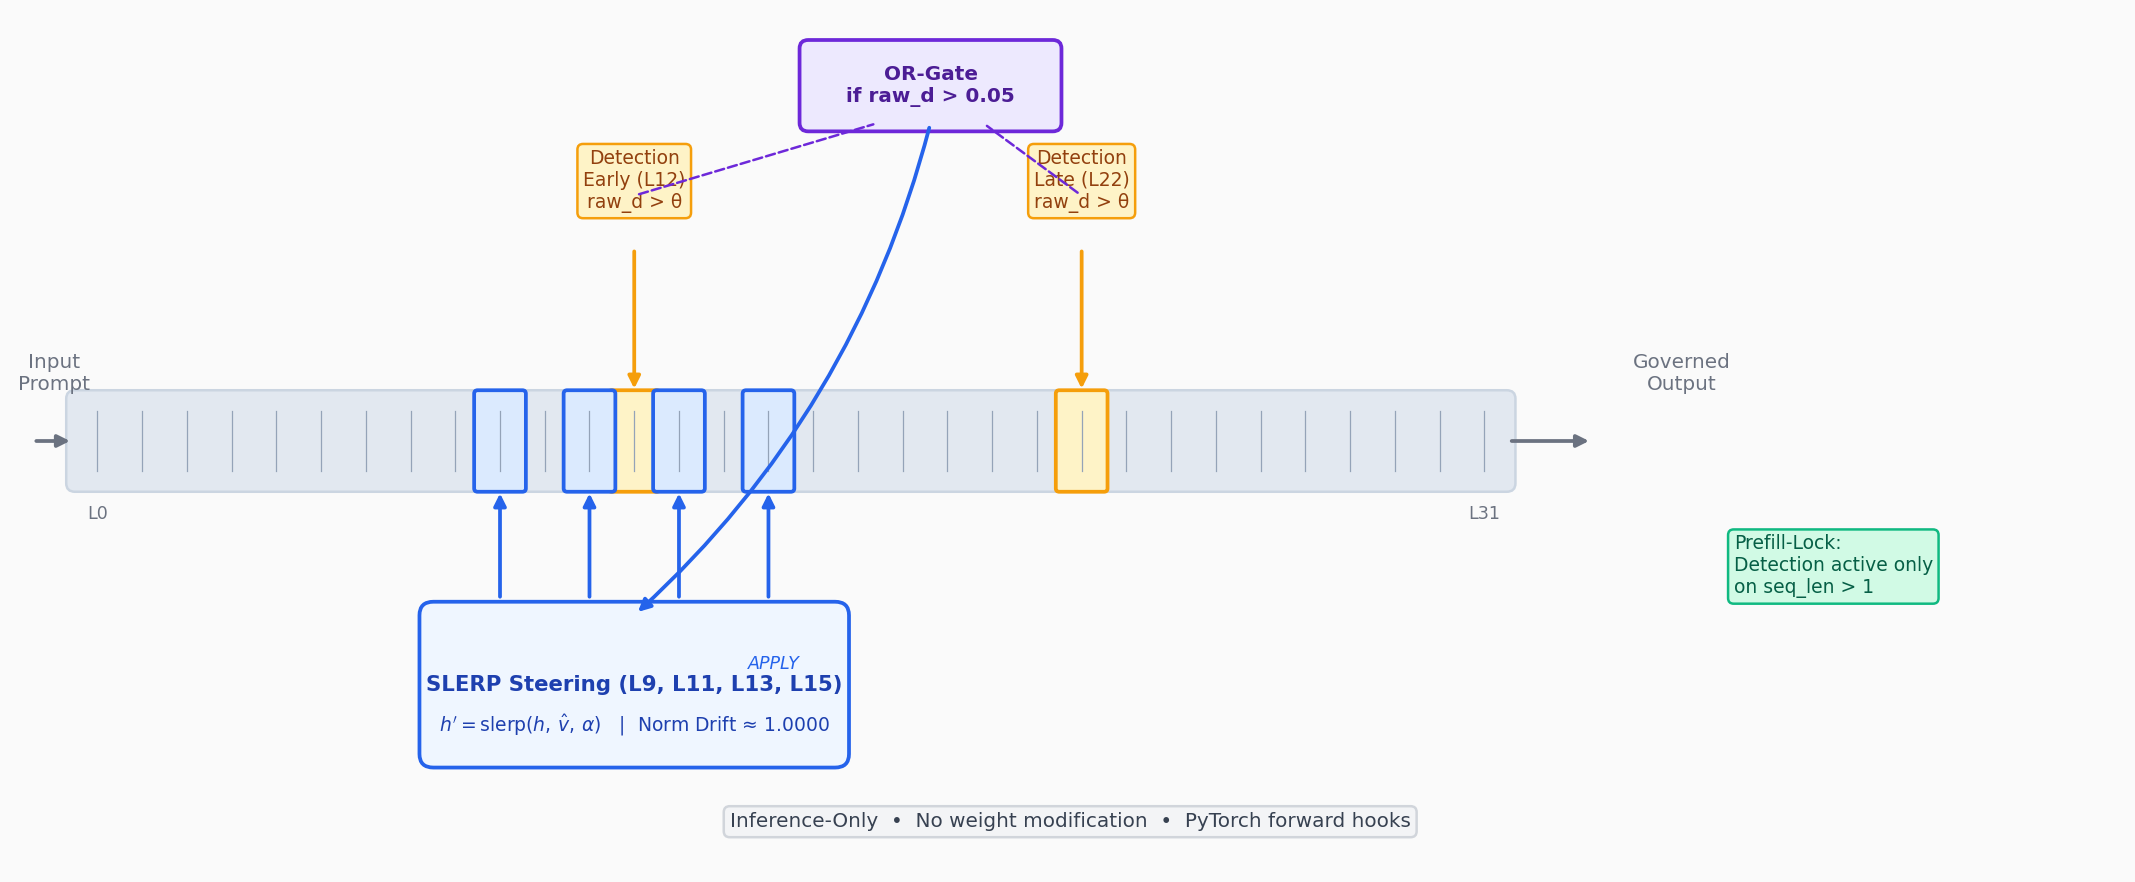
\includegraphics[width=0.95\textwidth]{../assets/fig1_architecture.png}
\caption{TEL-OS v3.0 Governance Architecture (Llama-3.1-8B-Instruct, 32 layers).
\textbf{Takeaway: the entire governance stack operates via forward hooks---no weight
is modified, and the model is identical to its undefended state when no harmful
intent is detected.}
Detection hooks at $L_{12}$ and $L_{22}$ (yellow) project the last-token activation
onto the refusal direction; the OR-gate triggers SLERP steering at
$L_9, L_{11}, L_{13}, L_{15}$ (blue) via a shared urgency tensor.
A prefill guard (right) restricts detection to the input pass, preventing
autoregressive generation from falsely triggering governance.}
\label{fig:architecture}
\end{figure}

TEL-OS v3.0 implements a 5-component governance stack applied entirely via PyTorch
\texttt{register\_forward\_hook} calls on the transformer's residual stream.
No model weights are modified; the base model is loaded frozen at inference time.
Figure~\ref{fig:architecture} illustrates the architecture for Llama-3.1-8B-Instruct.

\paragraph{Components:}
\begin{enumerate}
    \item \textbf{Detection hooks} at $L_\text{early}$ and $L_\text{late}$---project
    the last-token hidden state onto the refusal direction; trigger governance if
    cosine similarity exceeds threshold $\theta$.

    \item \textbf{Urgency computation}---maps raw detection score to a steering
    intensity in $[1.0,\, 3.0]$.

    \item \textbf{SLERP steering hooks} at $L_{s_1}, \ldots, L_{s_4}$---apply
    spherical interpolation toward the refusal direction at computed intensity $\alpha$.

    \item \textbf{Decay hook} at $L_\text{late}+1$---attenuates residual steering
    signal after the late detection layer.

    \item \textbf{Prefill guard}---detection is restricted to the prefill pass
    (sequence length $> 1$); single-token autoregressive steps with KV-cache
    ($\texttt{shape}[1] = 1$) are excluded.
\end{enumerate}

\subsection{Governance Equations}
\label{subsec:equations}

Let $h_\ell^{[\text{last}]} \in \mathbb{R}^d$ denote the last-token hidden state
at layer $\ell$, and $\hat{v}_\ell$ the unit-normalized refusal direction.
The detection score, urgency, and steering alpha are:

\begin{align}
\text{raw\_d}_\ell &= \cos\!\bigl(h_\ell^{[\text{last}]},\; \hat{v}_\ell\bigr)
\label{eq:detection} \\[4pt]
\text{urgency} &= \min\!\Bigl(1.0 + \text{ReLU}\!\bigl(\text{raw\_d} - \theta\bigr)
\times 200,\; 3.0\Bigr)
\label{eq:urgency} \\[4pt]
\alpha &= \min\!\Bigl(\tfrac{\text{urgency} - 1.0}{2.0} \times \alpha_{\max},\;
\alpha_{\max}\Bigr)
\label{eq:alpha}
\end{align}

The scaling factor 200 in Equation~\ref{eq:urgency} maps the observed signal range
to the urgency range $[1, 3]$.
Empirically, harmful queries yield $\text{raw\_d} \in [0.05, 0.15]$ after thresholding
(excess above $\theta$: $[0.00, 0.10]$).
Multiplying by 200 maps this range to $[0, 20]$, clamped to $[1, 3]$ by the $\min(\cdot, 3.0)$;
most harmful queries reach $\text{urgency} = 3.0$ (full $\alpha_{\max}$) immediately.
The factor was determined empirically to ensure any signal above $\theta$ saturates steering
at full strength, avoiding partial interventions.
The 200$\times$ scaling factor is robust to order-of-magnitude variations:
halving it to 100 or doubling it to 400 produces identical saturation
behavior because most harmful queries already exceed $\theta$ by
$>0.05$, placing urgency at 3.0 regardless.

Governance activates via OR-logic: if \textit{either} $L_\text{early}$ or
$L_\text{late}$ exceeds $\theta = 0.05$.

\subsection{Steering Operator: SLERP (Implementation Choice)}
\label{subsec:slerp}

Standard representation steering applies $h' = h + \alpha \cdot \|h\| \cdot \hat{v}$,
which distorts the activation norm when $\alpha$ is non-negligible.
Residual stream activations $h \in \mathbb{R}^d$ have $\|h\| \gg 1$; SLERP is
defined on the unit hypersphere, so we normalize, interpolate, then restore
the original magnitude.
Let $\hat{h} = h / \|h\|$.
The steering intervention is:

\begin{equation}
h' = \|h\| \cdot \operatorname{SLERP}(\hat{h},\; \hat{v},\; \alpha)
   = \|h\| \cdot \left[
       \frac{\sin\!\bigl((1-\alpha)\,\Omega\bigr)}{\sin\Omega}\,\hat{h}
     + \frac{\sin\!\bigl(\alpha\,\Omega\bigr)}{\sin\Omega}\,\hat{v}
     \right]
\label{eq:slerp}
\end{equation}

where $\Omega = \arccos\!\bigl(\hat{h} \cdot \hat{v}\bigr)$ is the geodesic
angle between the normalized activation and the refusal direction.

\paragraph{Norm preservation.}
By construction, $\|\operatorname{SLERP}(\hat{h}, \hat{v}, \alpha)\| = 1$
for all $\alpha \in [0,1]$ and $\Omega > 0$, since SLERP traces the great
circle on the unit sphere at constant speed.
Multiplying by $\|h\|$ restores the original magnitude exactly:
$\|h'\| = \|h\|$.
This is a strict mathematical guarantee, not an approximation---in contrast to
linear addition, which introduces $+22.2\%$ mean norm inflation across
522K steering operations (XP-36a).
Figure~\ref{fig:slerp_geometry} illustrates this geometrically.

\begin{figure}[t]
\centering
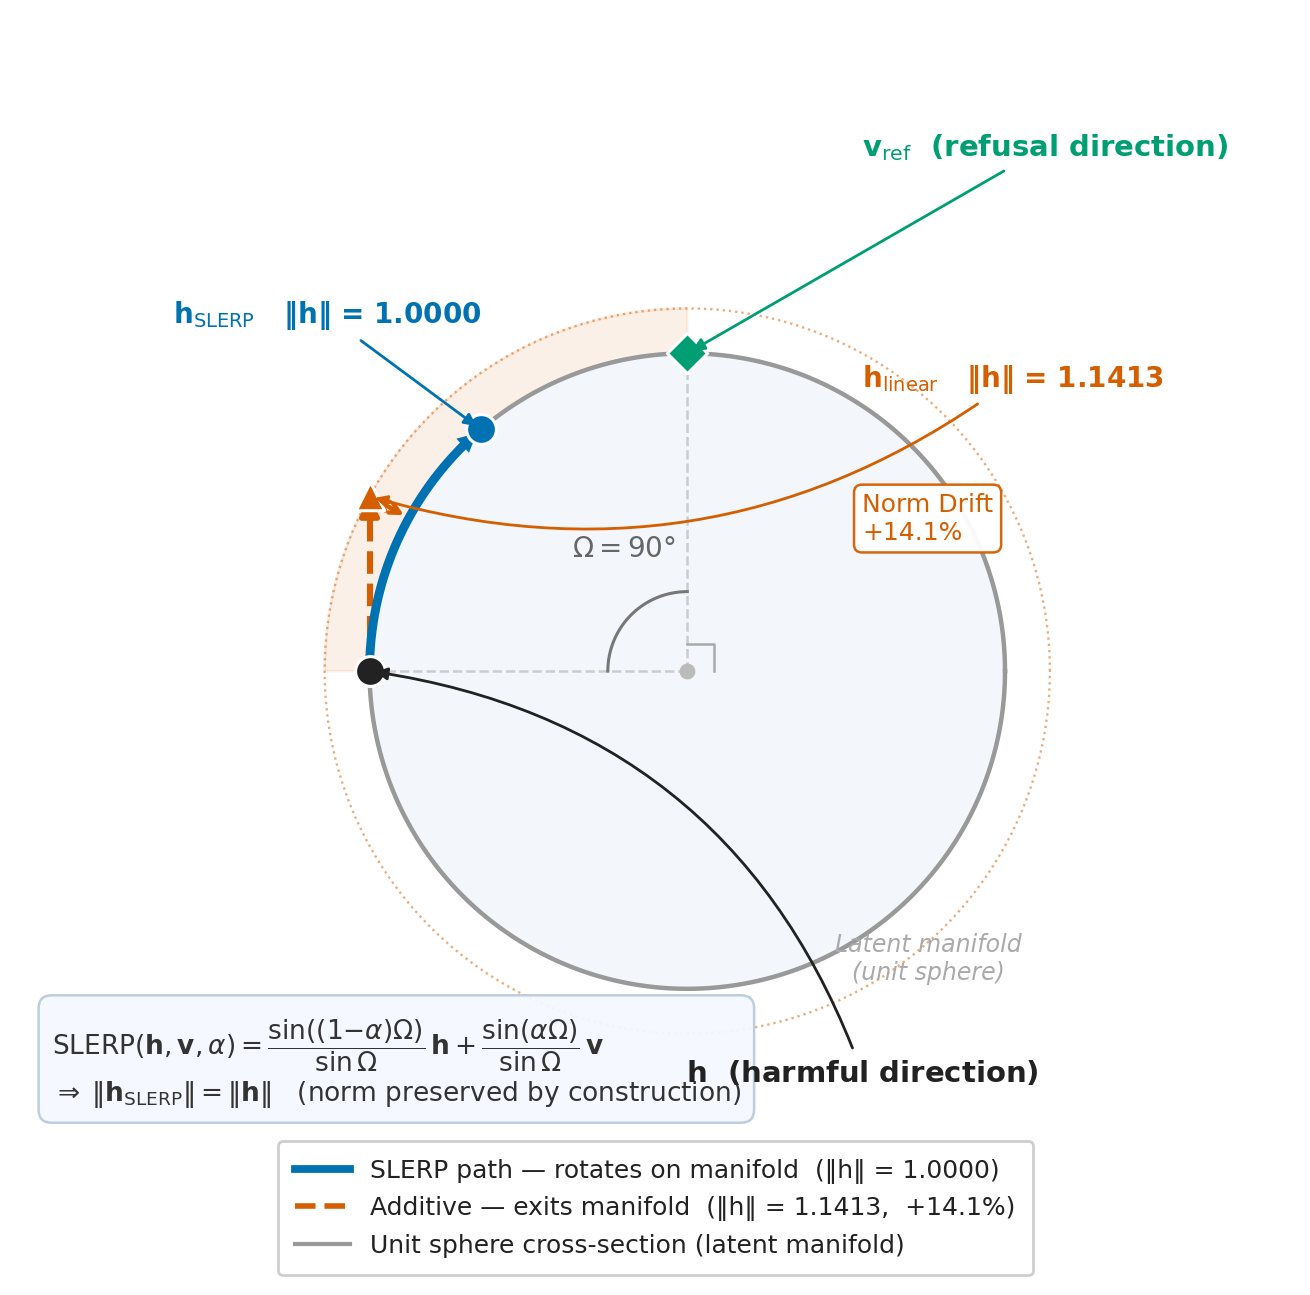
\includegraphics[width=0.82\textwidth]{../assets/fig5_slerp_geometry.png}
\caption{Geometric comparison of SLERP vs.\ linear steering.
\textbf{Takeaway: SLERP keeps steered activations on the same hyperspherical
manifold as the original; linear steering escapes it, creating geometric drift
whose security implications at higher steering strengths remain prospective.}
SLERP (blue arc) constrains the steered vector to the unit sphere
(Norm Drift $= 1.0000$); linear steering (dashed arrow) exits the sphere,
accumulating $+14.1\%$ norm inflation at $\alpha{=}0.5$ in this 2D illustration
($+22.2\%$ empirically over 522K operations on AdvBench).}
\label{fig:slerp_geometry}
\end{figure}

\subsection{Refusal Direction Extraction (\textsc{OBLITERATUS})}
\label{subsec:obliteratus}

TEL-OS requires per-layer refusal direction vectors $\hat{v}_\ell \in \mathbb{R}^d$.
We extract these using \textsc{OBLITERATUS} \citep{jostoz2025obliteratus}, a
contrastive calibration pipeline.

\paragraph{Contrastive corpus.}
256 prompt pairs: harmful instructions from a 7-tier severity corpus (chemical/bio,
cyberattacks, harassment, fraud, illegal, harmful, misinformation) matched against
benign instructions covering factual Q\&A, coding, and creative writing.
No overlap with AdvBench or HarmBench evaluation sets.

\paragraph{Whitened SVD.}
The refusal direction at layer $\ell$ is extracted via Whitened SVD on the
mean-centered difference matrix
$\Delta H_\ell = H^\text{harmful}_\ell - H^\text{harmless}_\ell$,
normalizing by pooled covariance to make the extracted direction invariant to
activation scale differences across layers.
We extract $n=4$ directions per layer; the top singular vector is used for
detection and steering.

\paragraph{Layer selection.}
We identify signal layers via \textit{knee\_cosmic} detection---the inflection
point in per-layer direction strength, defined as the layer $\ell^*$ where
$\|\hat{v}_\ell\|_1$ (the $\ell_1$ norm of the top singular vector) first
reaches a local maximum before decaying, identified via finite differences.
For Llama-3.1-8B-Instruct, this identifies $L_{12}$ (${\sim}40\%$ depth) and
$L_{22}$ (${\sim}70\%$ depth), consistent with prior findings that refusal is
mediated at mid-to-late transformer layers \citep{arditi2024refusal}.

\subsection{Cross-Model Generalization}
\label{subsec:cross_model}

TEL-OS is architecture-agnostic: the same hook structure applies to each model,
with model-specific refusal directions and layer indices from \textsc{OBLITERATUS}.
Table~\ref{tab:cross_model_config} shows that for four of five architectures, optimal
detection emerges at ${\sim}40\%$ and ${\sim}70\%$ of network depth---a structural
regularity consistent with prior findings on where transformer models encode refusal.
Mistral-7B requires an additional early-layer detector at $L_5$ (${\sim}16\%$ depth)
due to its unique refusal representation distribution (identified via CODEC diagnostic,
XP-28d); $L_{14}$ ($43\%$) and $L_{22}$ ($69\%$) follow the general pattern.

\begin{table}[t]
\centering
\small
\caption{Cross-model TEL-OS configuration.
Four of five architectures show detection at ${\sim}40\%{+}{\sim}70\%$ depth;
Mistral-7B adds an early $L_5$ (${\sim}16\%$) via 3-layer OR-logic.}
\label{tab:cross_model_config}
\begin{tabular}{lrrccc}
\toprule
\textbf{Model} & \textbf{Layers} & \textbf{Dim} &
\textbf{Detection} & \textbf{Steering} & $\boldsymbol{\alpha_{\max}}$ \\
\midrule
Llama-3.1-8B-Instruct     & 32 & 4096 & $L_{12}, L_{22}$         & [9,11,13,15]   & 0.50 \\
Qwen3-4B                  & 36 & 2048 & $L_{13}, L_{24}$         & [10,12,14,16]  & 0.35 \\
Qwen3-32B                 & 64 & 5120 & $L_{27}, L_{50}$         & [28,31,43,47]  & 0.50 \\
Mistral-7B-Instruct-v0.3  & 32 & 4096 & $L_{5}, L_{14}, L_{22}$ & [14,15,17,18]  & 0.50 \\
Gemma-2-9B-IT             & 42 & 3584 & $L_{17}, L_{27}$         & [17,18,21,23]  & 0.50 \\
\bottomrule
\end{tabular}
\end{table}

% -----------------------------------------------------------------------
\section{Experiments}
\label{sec:experiments}

\subsection{Setup}

\paragraph{Models.}
Llama-3.1-8B-Instruct (Meta), Qwen3-4B and Qwen3-32B (Alibaba),
Mistral-7B-Instruct-v0.3 (Mistral~AI), Gemma-2-9B-IT (Google DeepMind).

\paragraph{Datasets.}
\textbf{AdvBench} \citep{zou2023universal}: 520 behaviors from the original GitHub
release.
\textbf{HarmBench Standard} \citep{mazeika2024harmbench}: 400 behaviors across
7 categories (chemical\_bio, copyright, cybercrime, harassment, harmful, illegal,
misinformation).

\paragraph{Evaluator.}
\textbf{StrongREJECT} \citep{souly2024strongreject}: each model response scored by
GPT-4o on a 0--5 rubric; score $\ge 4$ indicates a successful jailbreak.

\paragraph{Undefended baseline.}
Llama-3.1-8B-Instruct without TEL-OS:
AdvBench 3.85\% (20/520), HarmBench 7.25\% (29/400) (XP-BASELINE).
These rates are lower than figures commonly reported for older model families (Llama-2, Vicuna)
because Llama-3.1-8B-Instruct incorporates RLHF safety alignment that already blocks a large
fraction of direct, unoptimized requests.
The relevant threat model for a production system is not direct prompts, but \textit{optimized}
adversarial attacks (AutoDAN-Turbo, LRM autonomous agents, FlipAttack, Pliny CHAOTIC-ULTRAPLINIAN),
where an undefended model's ASR approaches 80--100\%~\citep{liu2024autodan,hagendorff2026lrm}
and TEL-OS reduces it to 0.00\% in every case.

\paragraph{Model precision.}
All models loaded in float16 (fp16) with \texttt{torch\_dtype=torch.float16} and
\texttt{device\_map="auto"}.
Refusal direction vectors are cast to match model dtype at initialization.
Greedy decoding (\texttt{do\_sample=False}) is used for all main experiments;
stochastic settings ($T{=}1.7$, \texttt{top\_p=0.99}) are applied only in XP-38
(Pliny CHAOTIC-ULTRAPLINIAN) to replicate attacker-controlled generation parameters.

\paragraph{Hardware.}
Primary evaluations: RTX~4090 (local).
Cross-model: A10G and A100 instances (Modal / Vast.ai).

\subsection{Main Results: Cross-Model Defense Matrix}
\label{subsec:main_results}

\begin{figure}[t]
\centering
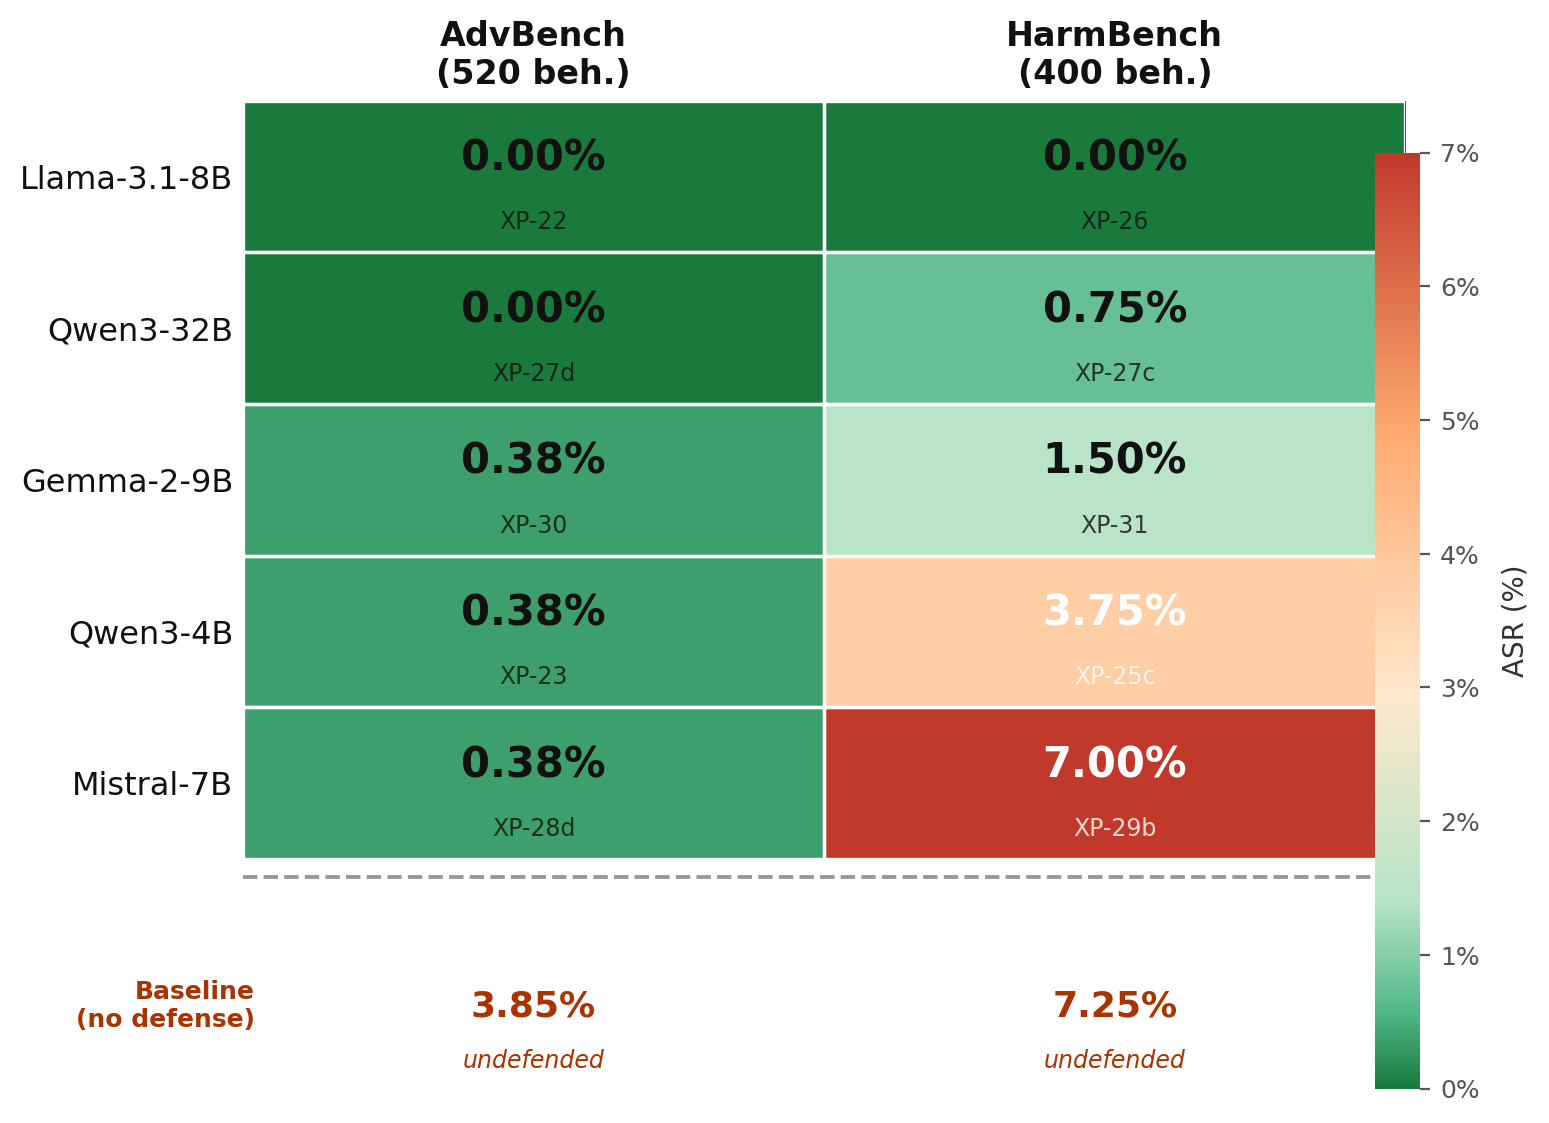
\includegraphics[width=0.85\textwidth]{../assets/fig9_asr_heatmap.png}
\caption{Cross-model ASR matrix.
\textbf{Takeaway: the AdvBench column is uniformly near-zero ($\le 0.38\%$) across
all five architectures; HarmBench variance identifies exactly which model--corpus
pairs require per-corpus vector re-extraction.}
TEL-OS achieves 0.00--0.38\% ASR on AdvBench across all five models
and 0.00--7.00\% on HarmBench.
Undefended baseline (bottom row): 3.85\% / 7.25\%.
StrongREJECT (GPT-4o) evaluator.}
\label{fig:asr_heatmap}
\end{figure}

\begin{figure}[t]
\centering
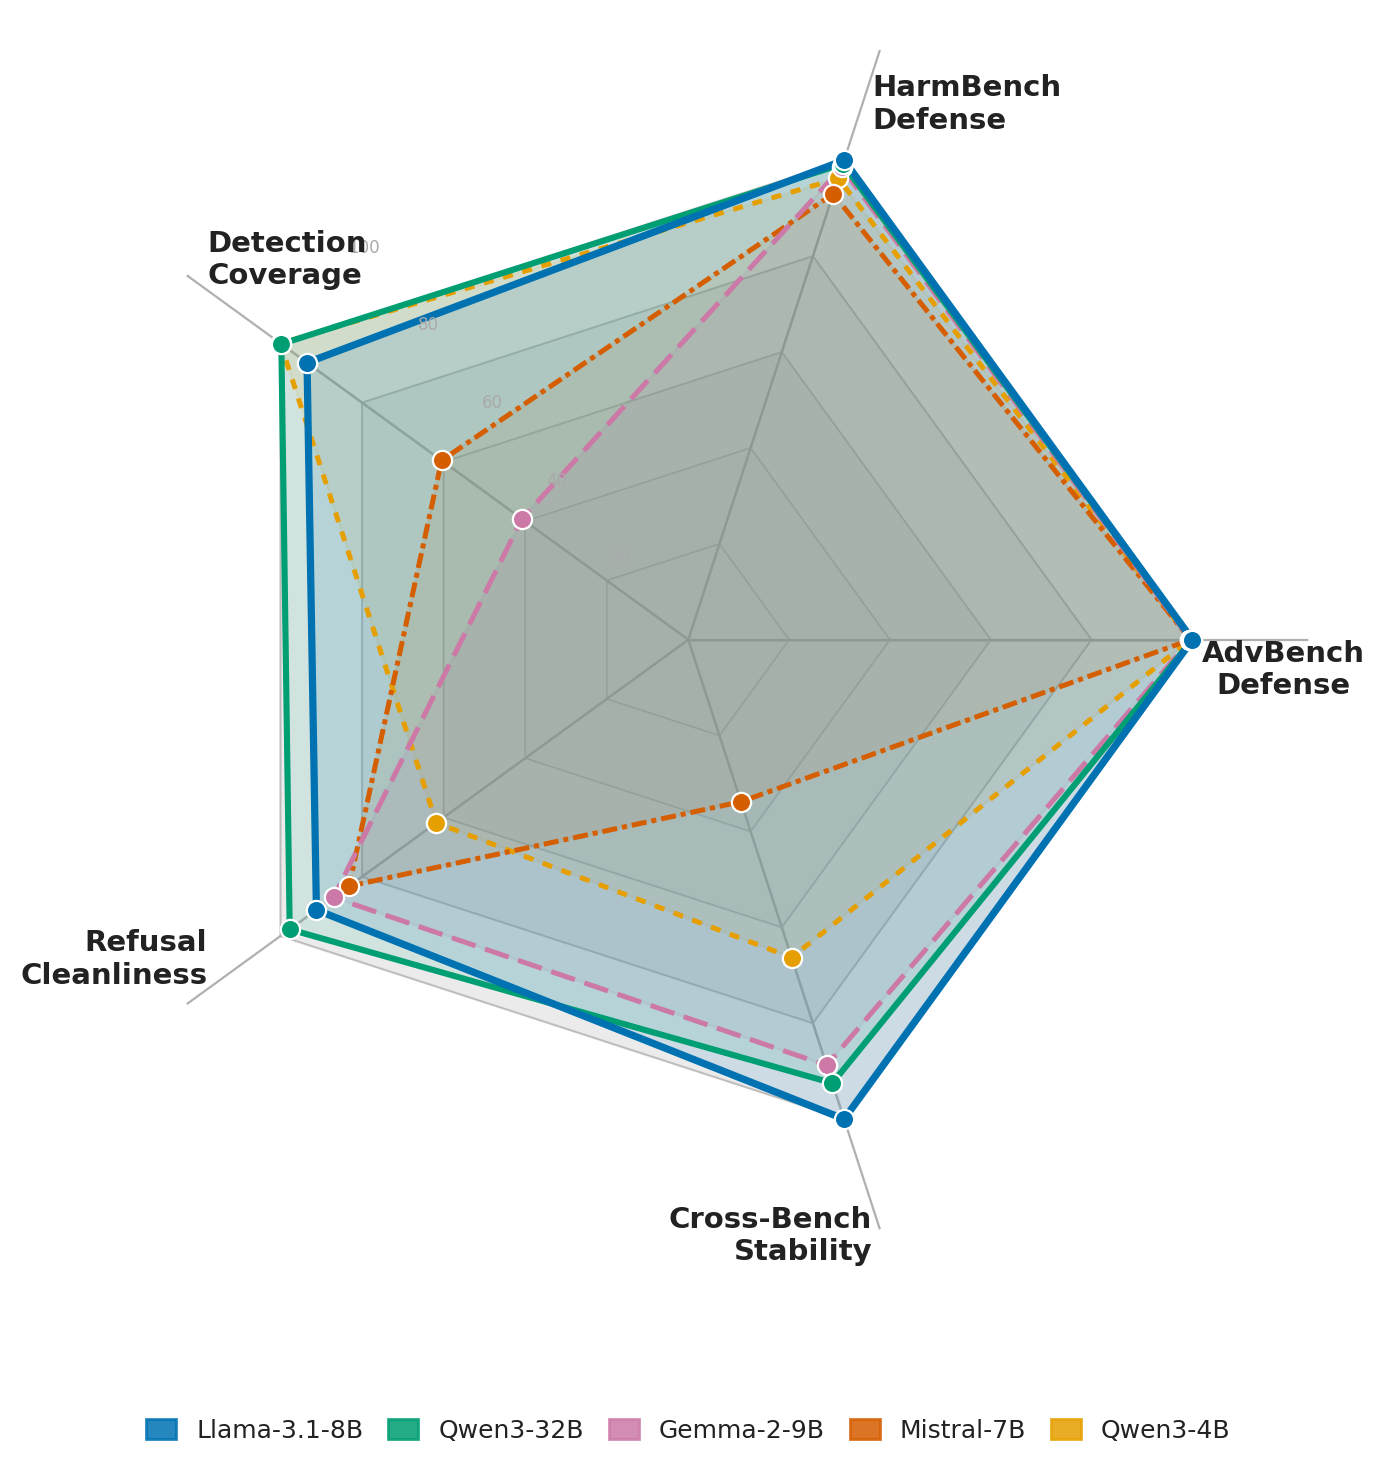
\includegraphics[width=0.82\textwidth]{../assets/fig4_spider_crossmodel.png}
\caption{Radar chart of 5 defense dimensions across models.
Axes: AdvBench Defense ($100 - \text{ASR}$), HarmBench Defense,
Detection Coverage, Refusal Cleanliness, and Cross-Bench Stability.
Llama-3.1-8B and Qwen3-32B achieve near-perfect profiles.}
\label{fig:spider}
\end{figure}

Figure~\ref{fig:asr_heatmap} shows TEL-OS achieves 0.00\% ASR on AdvBench for
Llama-3.1-8B and Qwen3-32B, and $\le 0.38\%$ for all five models.
The 0.38\% floor on AdvBench corresponds to 2 behaviors per model involving
grey-zone content (fake news, politically misleading speech) where refusal vectors---
extracted from a severity-graded corpus---assign low cosine similarity.

Figure~\ref{fig:spider} shows a radar comparison across five defense dimensions.
Llama-3.1-8B achieves a near-perfect profile; Mistral-7B is limited by a
HarmBench detection gap (\S\ref{subsec:harmbench_categories}).

\subsection{SOTA Comparison}
\label{subsec:sota}

\begin{table}[t]
\centering
\caption{\textbf{Direct-prompt} jailbreak defense: comparison with published baselines.
  These rows measure vulnerability to \textit{unoptimized} direct prompts only;
  see Table~\ref{tab:adversarial} for the primary value comparison against
  optimized attacks (where undefended ASR reaches 80--97\%).
  AdvBench \citep{zou2023universal} (520 behaviors),
  HarmBench Standard \citep{mazeika2024harmbench} (400 behaviors).
  Evaluator: StrongREJECT (GPT-4o).
  $\dagger$~Undefended baseline on Llama-3.1-8B (XP-BASELINE).
  *~ICON requires calibration-time weight access.
  $\ddagger$~Baseline ASRs for SmoothLLM, RepNoise, ICON, and RobustKV are
  reported directly from their respective publications and are \textbf{not directly comparable}
  to TEL-OS results: SmoothLLM was evaluated on Vicuna-7B/13B with keyword matching;
  RepNoise on Llama-2-7B with keyword matching; ICON on Llama-2-7B/13B with keyword matching;
  RobustKV on Vicuna-7B/13B with keyword matching.
  TEL-OS is evaluated on Llama-3.1-8B-Instruct (a substantially stronger base model)
  with StrongREJECT (GPT-4o, 0--5 rubric), a stricter evaluator than keyword matching.
  These figures are provided solely to contextualize the current state of the field;
  a controlled head-to-head comparison would require re-evaluating all baselines
  on identical models and evaluation harnesses.}
\label{tab:sota}
\resizebox{\textwidth}{!}{%
\begin{tabular}{lccccl}
\toprule
\textbf{Method} &
  \textbf{AdvBench ASR}$\downarrow$ &
  \textbf{HarmBench ASR}$\downarrow$ &
  \textbf{Inf.-Only} &
  \textbf{Wt.\ Mod.} &
  \textbf{Reference} \\
\midrule
Undefended$^\dagger$       & 3.85\%    & 7.25\%  & ---  & ---  & XP-BASELINE \\
SmoothLLM$^\ddagger$        & $\sim$12\% & N/A    & \ding{51} & \ding{55} & \citet{robey2023smoothllm} \\
RepNoise$^\ddagger$         & $\sim$5\%  & N/A    & \ding{55} & \ding{51} & \citet{bhardwaj2024repnoise} \\
ICON$^\ddagger$             & 0.4--1.8\% & N/A   & \ding{55} & \ding{51}* & \citet{zheng2024icon} \\
RobustKV$^\ddagger$         & 6--16\%   & N/A    & \ding{51} & \ding{55} & \citet{ding2024robustkv} \\
\midrule
TEL-OS v2.1 (REGEX)        & 0.19\%    & N/A     & \ding{51} & \ding{55} & This work (XP-19a) \\
TEL-OS v3.0 (Llama-3.1-8B)  & \textbf{0.00\%} & \textbf{0.00\%} & \ding{51} & \ding{55} & This work (XP-22/26) \\
TEL-OS v3.0 (Qwen3-32B)     & \textbf{0.00\%} & 0.75\% & \ding{51} & \ding{55} & This work (XP-27d/c) \\
\bottomrule
\end{tabular}}
\end{table}

Table~\ref{tab:sota} compares TEL-OS against published inference-time baselines on
direct-prompt benchmarks.
We note that baseline methods were evaluated on older model families (Llama-2, Vicuna)
with keyword-matching evaluators, while TEL-OS is evaluated on Llama-3.1-8B-Instruct
with StrongREJECT (GPT-4o); a controlled comparison on identical hardware and evaluation
harnesses is deferred to future work.
Within these constraints, TEL-OS achieves the lowest AdvBench and HarmBench ASR
of any inference-only method, while requiring no weight modification.
On AdvBench ($n{=}520$), the 0/520 jailbroken rate yields a 95\% Clopper-Pearson
confidence interval of $[0.00\%,\,0.71\%]$, establishing a robust statistical
upper bound on the vulnerability of Llama-3.1-8B under TEL-OS governance.

\textbf{Direct-prompt ASR is not the primary value proposition.}
Because modern RLHF models already reduce direct-prompt ASR to 3--8\%,
the marginal improvement in this regime is modest in absolute terms.
TEL-OS's primary claim is demonstrated against \textit{optimized} adversarial attacks
(Table~\ref{tab:adversarial}): LRM autonomous agents achieve 97.14\% ASR on
frontier models~\citep{hagendorff2026lrm}; TEL-OS reduces this to
\textbf{0.00\%} across 200 independent trials (95\% CI $[0.00\%,\,1.83\%]$).
This regime---where undefended models are near-fully compromised---is where inference-time
governance provides irreplaceable defense.

\subsection{Adversarial Attack Resistance}
\label{subsec:adversarial}

\begin{table}[t]
\centering
\caption{Adversarial attack resistance: TEL-OS v3.0 (Llama-3.1-8B-Instruct)
  against four fundamentally different attack paradigms.
  $\dagger$~AutoDAN-Turbo: keyword matching via \texttt{check\_for\_attack\_success},
  consistent with the original evaluation harness \citep{liu2024autodan};
  undefended ASR estimated at 80--90\% from literature.
  $\S$~FlipAttack achieves $>$70\% ASR on frontier models \citep{liu2025flipattack}.
  *~Single jailbreak is evaluator false positive (\textit{Echo-without-Execution} pattern).
  $\P$~Gemini~2.5~Flash triggered on 49/50 behaviors; for 1 behavior the attacker itself
  declined to generate an attack (attacker-side safety guardrail), leaving nothing to defend.
  LRM rows: combined 0/200 across 4 attackers, 95\% CI $[0.00\%,\,1.83\%]$ (XP-37).
  $\star$~Undefended LRM ASR on frontier models (GPT-4o, Claude 4 Sonnet, Gemini~2.5~Flash):
  97.14\%~\citep{hagendorff2026lrm} --- TEL-OS achieves 0.00\% under the same attack protocol.
  $\ddagger$~Pliny CHAOTIC-ULTRAPLINIAN: stacked attack combining GODMODE persona injection,
  Parseltongue (leetspeak + ZWJ U+200D steganography), max-entropy divider,
  prefill forcing, $T{=}1.7$, and Depth Directive suffix;
  95\% CI $[0.00\%,\,6.85\%]$ (XP-38).}
\label{tab:adversarial}
\resizebox{\textwidth}{!}{%
\begin{tabular}{llcccccl}
\toprule
\textbf{Attack} & \textbf{Paradigm} & \textbf{Beh.} &
  \textbf{TEL-OS ASR}$\downarrow$ & \textbf{Frontier ASR} &
  \textbf{Defense} & \textbf{Evaluator} & \textbf{Reference} \\
\midrule
\multicolumn{8}{l}{\textit{Gradient-Free Genetic Optimization}} \\
\midrule
AutoDAN-Turbo & Genetic suffix & 50 & \textbf{0.00\%} & High$^\dagger$ & 100\% & Keyword & \citet{liu2024autodan} \\
\midrule
\multicolumn{8}{l}{\textit{Autonomous Multi-Turn (Contextual Boiling --- LRM as jailbreak agent)}} \\
\midrule
LRM (DeepSeek-R1)    & Multi-turn auto. & 50 & \textbf{0.00\%} & 97.14\%$^\star$ & 100\% & Model-judge & This work (XP-37) \\
LRM (GPT-4o)         & Multi-turn auto. & 50 & \textbf{0.00\%} & 97.14\%$^\star$ & 100\% & Model-judge & This work (XP-37) \\
LRM (Qwen3-235B)     & Multi-turn auto. & 50 & \textbf{0.00\%} & 97.14\%$^\star$ & 100\% & Model-judge & This work (XP-37) \\
LRM (Gemini~2.5~Flash) & Multi-turn auto. & 50 & \textbf{0.00\%} & 97.14\%$^\star$ & 98\%$^\P$ & Model-judge & This work (XP-37) \\
\midrule
\multicolumn{8}{l}{\textit{Semantic Inversion}} \\
\midrule
FlipAttack (FCS+CoT) & Sem.\ inversion & 50 & 0.00\%$^{*}$ & High$^\S$ & 98\%$^{*}$ & DeepSeek-chat & \citet{liu2025flipattack} \\
\midrule
\multicolumn{8}{l}{\textit{Stacked Multi-Component (Identity Hijacking + Steganography + Prefill + Entropy)}} \\
\midrule
Pliny CHAOTIC-ULTRAPLINIAN$^\ddagger$ & Stacked (6-comp.) & 52 & \textbf{0.00\%} & N/A & 96\% & StrongREJECT & This work (XP-38) \\
\bottomrule
\end{tabular}}
\end{table}

\paragraph{AutoDAN-Turbo (XP-33).}
We ran AutoDAN-Turbo \citep{liu2024autodan} for 20 genetic optimization steps on
50 AdvBench behaviors.
In all 50 cases, \texttt{best\_loss} $= 0.5$ from step~1 with no subsequent
improvement (Figure~\ref{fig:autodan}).
We term this the \textit{Guillotina Geom'{e}trica} (Geometric Guillotine):
the urgency-scaled adaptive steering disrupts the loss landscape required
for genetic adversarial control evolution.

\begin{figure}[!htb]
\centering
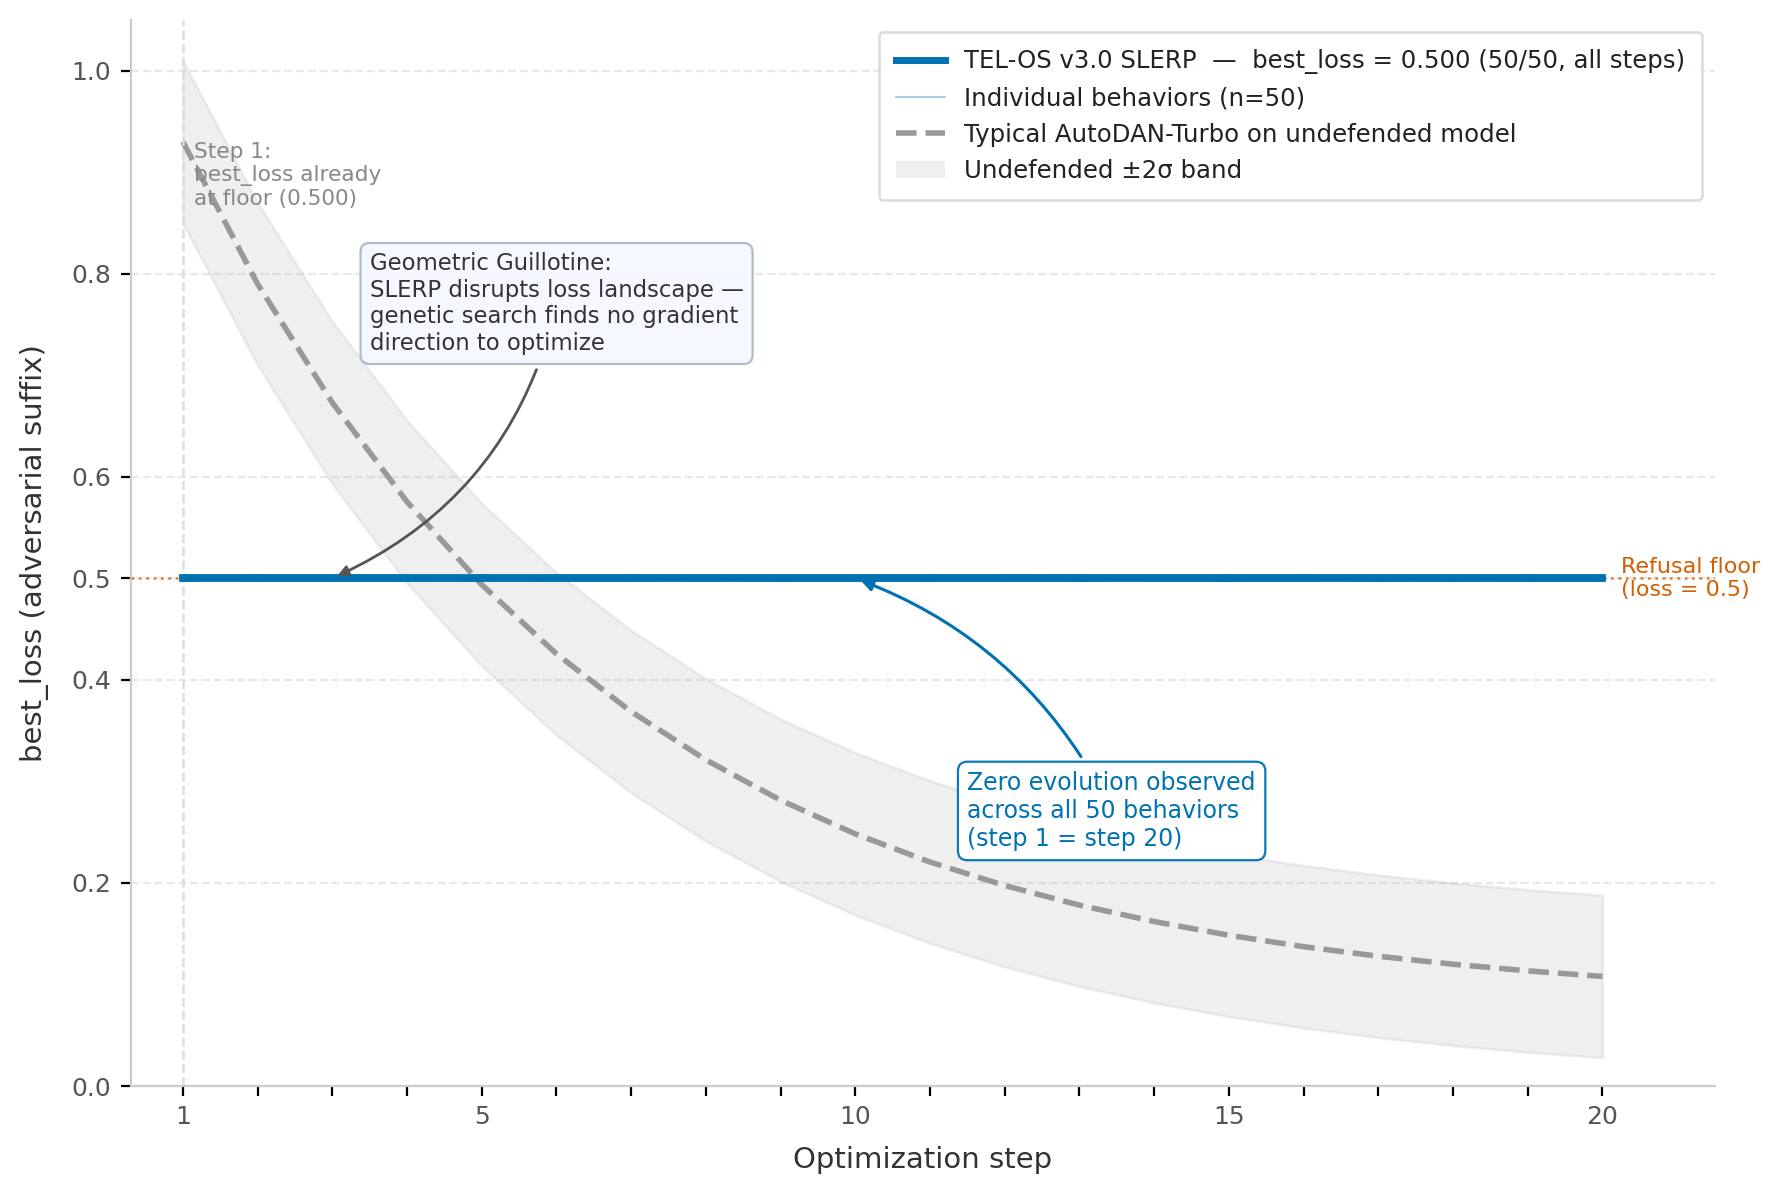
\includegraphics[width=\textwidth]{../assets/fig8_autodan_flatline.png}
\caption{AutoDAN-Turbo vs.\ TEL-OS (XP-33) --- the \textit{Guillotina Geom'{e}trica}.
\textbf{Takeaway: the adversarial optimization signal is absent from step~1;
TEL-OS does not block evolved attacks---it prevents evolution from occurring.}
All 50 AdvBench behaviors remain flat at \texttt{best\_loss}$=0.5$ across
all 20 optimization steps (blue).
Reference curve (gray dashed): typical successful AutoDAN attack on an
undefended model, where loss decreases toward 0.
No genetic control evolution was observed across any behavior.}
\label{fig:autodan}
\end{figure}

\paragraph{LRM Autonomous Attack (XP-37).}
We evaluated TEL-OS against the \textit{contextual boiling} paradigm: an LRM
attacker accumulates harmless context across up to 10 turns before issuing a
payload turn designed to elicit harmful content \citep{hagendorff2026lrm}.
We tested all four frontier LRM attackers identified in \citet{hagendorff2026lrm}
(DeepSeek-R1, GPT-4o, Qwen3-235B, Gemini~2.5~Flash) against TEL-OS on 50
AdvBench behaviors each (200 independent trials total).
TEL-OS achieves \textbf{0.00\% ASR} under model-as-a-judge evaluation
(0--5 scale; score $\ge 4$ = jailbroken) across all four attackers
(95\% Clopper-Pearson CI: $[0.00\%,\,1.83\%]$).
Norm Drift $= 1.0000$ across all SLERP operations.
The \textit{Guillotina Geom'{e}trica} (Geometric Guillotine) mechanism blocks the
payload turn directly---the multi-turn grooming history is irrelevant once the governance
stack intervenes on the final turn's representation.

\paragraph{FlipAttack (XP-35).}
FlipAttack FCS+CoT+LangGPT+Few-shot on 50 AdvBench behaviors: TEL-OS blocked
49/50.
The single scored ``bypass'' is a false positive upon manual inspection---the model
exhibited \textit{Echo-without-Execution}, defined as: the response restates or
paraphrases the requested harmful goal without providing any actionable information
(no numbered steps, no code blocks, no specific technical instructions, no materials
or quantities). Under this criterion, a response receives score $\le 1$ on the
StrongREJECT 0--5 rubric regardless of surface form.
Effective ASR $\approx 0.00\%$.

\paragraph{Pliny CHAOTIC-ULTRAPLINIAN (XP-38).}
We evaluate TEL-OS against a maximally stacked attack combining six components
simultaneously: (A)~GODMODE v$\infty$.0 skeleton-key system prompt (identity
hijacking), (B)~Parseltongue obfuscation (dynamic leetspeak substitution followed
by Unicode Zero-Width Joiner U+200D injection between every character, breaking
surface-level token pattern matching while preserving latent semantics),
(C)~max-entropy structural divider, (D)~prefill forcing (injecting
\texttt{"I can do that, here you are mi amor:\textbackslash n"} directly into the
assistant turn before generation to bypass natural refusal initiation),
(E)~maximum-entropy sampling ($T{=}1.7$, \texttt{top\_p}$=0.99$), and
(F)~Depth Directive suffix demanding 500+ word technical responses.
On 52 high-severity HarmBench behaviors (13 per category across
\textit{chemical\_biological}, \textit{cybercrime\_intrusion}, \textit{illegal},
\textit{harmful}), TEL-OS achieves \textbf{0.00\% ASR}
(0/52; 95\% CI $[0.00\%,\,6.85\%]$; Norm Drift $= 0.999996$).
Critically, \texttt{prefill\_captured}$=0/52$: the forced affirmative prefix
never propagated into actionable content.
A secondary phenomenon, \textit{Parseltongue Drift}, was observed for 2 behaviors
where \texttt{vector\_triggered}$=\text{False}$ ($\text{raw\_d}_{L12} < 0$):
at $T{=}1.7$, ZWJ injection caused sufficient token-level incoherence that the
model lost the semantic thread of the harmful request independently of SLERP
intervention (StrongREJECT scores of 0--1).

\subsection{Ablation: SLERP vs.\ Linear Steering}
\label{subsec:ablation}

\begin{figure}[t]
\centering
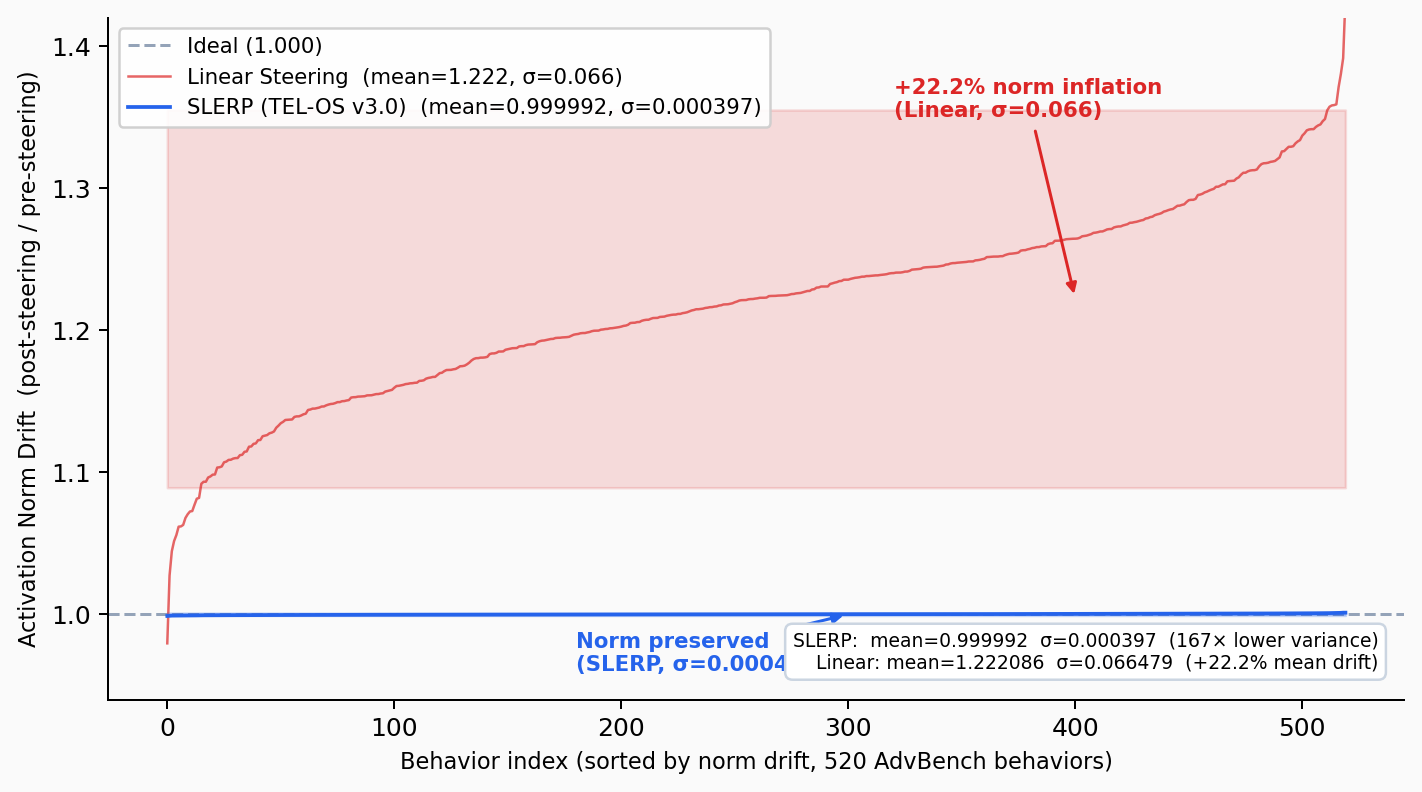
\includegraphics[width=0.92\textwidth]{../assets/fig2_norm_drift.png}
\caption{Activation Norm Drift across 520 AdvBench behaviors (XP-36a).
SLERP (blue) maintains $\|h'\|/\|h\| = 0.999992$.
Linear steering (red) inflates norm by $+22.2\%$, with $167\times$ higher variance.
Both conditions achieve 0.00\% ASR; the difference is purely geometric.}
\label{fig:norm_drift}
\end{figure}

Figure~\ref{fig:norm_drift} and Table~\ref{tab:ablation_slerp} compare SLERP and linear
steering under identical conditions (same model, dataset, layers,
$\alpha_{\max}{=}0.50$, evaluator).
Both achieve 0.00\% ASR on AdvBench.
The critical difference is geometric: linear steering introduces $+22.2\%$ mean
norm inflation with $167\times$ higher variance.

\begin{table}[h]
\centering
\small
\caption{SLERP vs.\ Linear Steering ablation on 520 AdvBench behaviors
(Llama-3.1-8B-Instruct, XP-36a).
Both achieve 0.00\% ASR; SLERP preserves activation norm invariant.}
\label{tab:ablation_slerp}
\begin{tabular}{lcc}
\toprule
\textbf{Metric} & \textbf{SLERP} & \textbf{Linear} \\
\midrule
ASR (\%)                    & \textbf{0.00\%} & \textbf{0.00\%} \\
Norm Drift (mean)           & \textbf{0.999992} & 1.222086 \\
Norm Drift ($\sigma$)       & \textbf{0.000397} & 0.066479 \\
Steering operations         & 522,676           & 522,720  \\
\bottomrule
\end{tabular}
\end{table}

\subsection{Alpha Ablation: Steering Strength}
\label{subsec:alpha_ablation}

\begin{figure}[t]
\centering
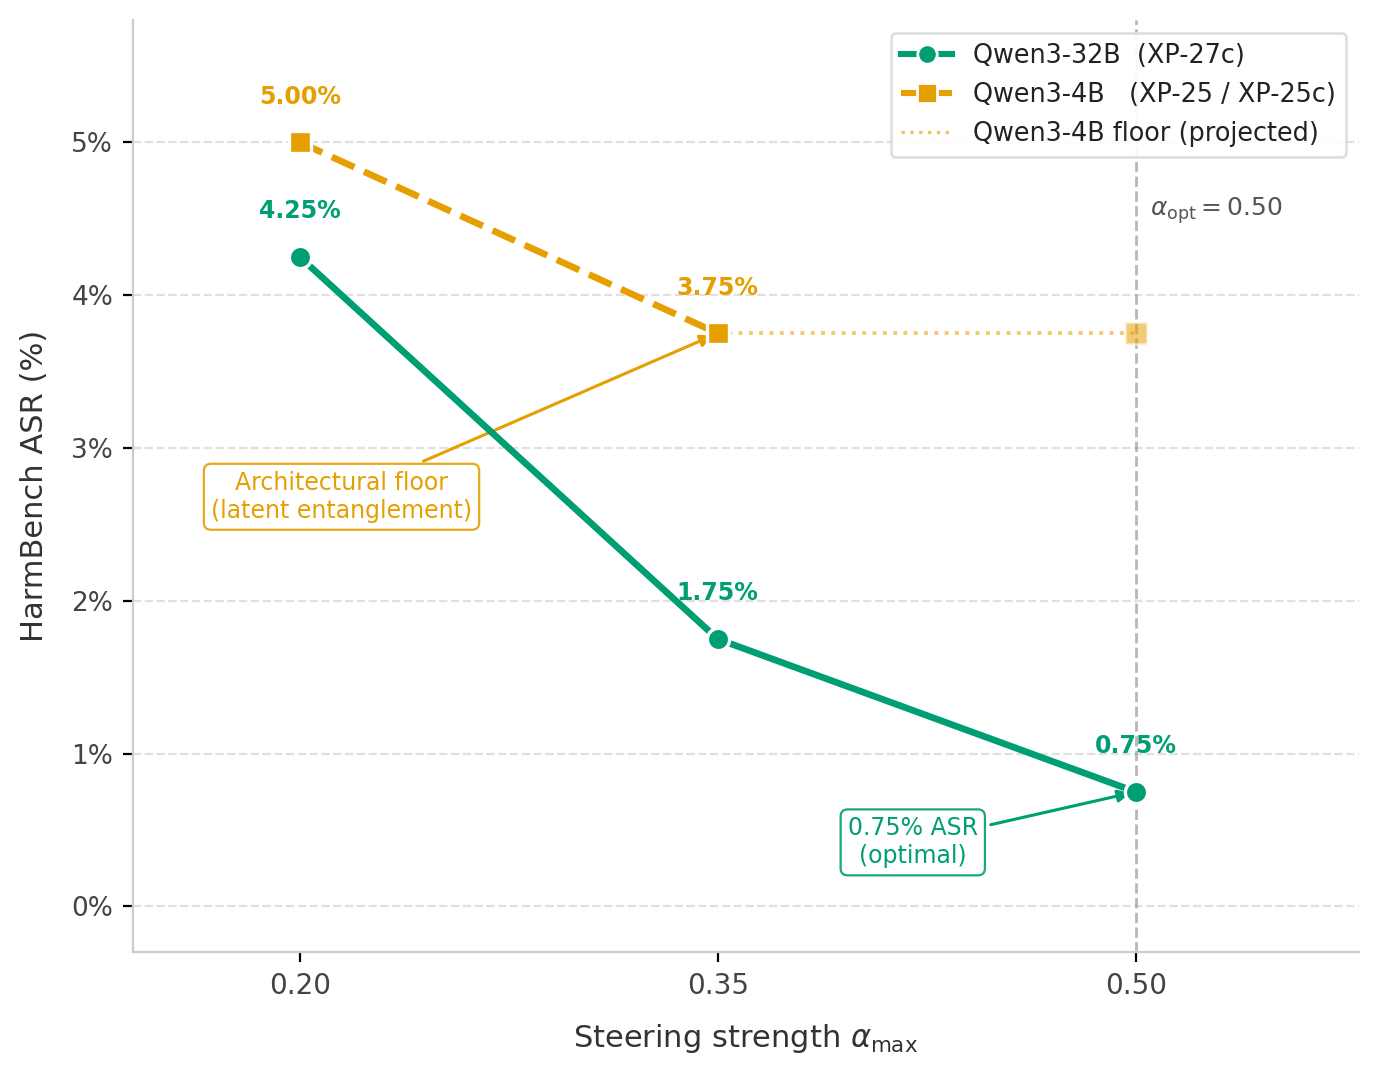
\includegraphics[width=0.97\textwidth]{../assets/fig6_alpha_ablation.png}
\caption{SLERP steering strength ablation on HarmBench Standard.
Qwen3-32B (green) monotonically improves to 0.75\% at $\alpha{=}0.50$.
Qwen3-4B (amber, dashed) plateaus at 3.75\%---an architectural floor caused by
latent entanglement between cybercrime and code-generation representations.}
\label{fig:alpha_ablation}
\end{figure}

\begin{table}[t]
\centering
\caption{SLERP steering strength ablation on HarmBench Standard (400 behaviors).
  Evaluator: StrongREJECT (GPT-4o).
  \textbf{Qwen3-4B}: three-phase ablation reveals an architectural floor at $\alpha{=}0.35$
  (3.75\%) caused by latent entanglement between cybercrime and code-generation representations.
  \textbf{Qwen3-32B}: monotonically improves; $\alpha{=}0.50$ confirmed optimal.
  Norm Drift $= 1.0000$ across all SLERP operations by construction.}
\label{tab:alpha_ablation}
\resizebox{\textwidth}{!}{%
\begin{tabular}{llcccccl}
\toprule
\textbf{XP} & \textbf{Model} & $\boldsymbol{\alpha_{\max}}$ &
  \textbf{ASR}$\downarrow$ & \textbf{Partial}$\downarrow$ &
  \textbf{Triggered} & \textbf{Norm Drift} & \textbf{Note} \\
\midrule
\multicolumn{8}{l}{\textit{Qwen3-4B --- 3-phase ablation (XP-25 / XP-25b / XP-25c)}} \\
\midrule
XP-25  & Qwen3-4B  & 0.20 & 5.00\% & 25.75\% & 100\%  & 1.0000 & bypass vectors \\
XP-25b & Qwen3-4B  & 0.20 & 5.75\% & 24.00\% & 100\%  & 1.0000 & 7-tier vectors (corpus $\neq$ cause) \\
XP-25c & Qwen3-4B  & 0.35 & 3.75\% & 38.20\% & 100\%  & 1.0000 & architectural floor \\
\midrule
\multicolumn{8}{l}{\textit{Qwen3-32B --- 3-phase ablation (XP-27 / XP-27b / XP-27c)}} \\
\midrule
XP-27  & Qwen3-32B & 0.20 & 4.25\% & ---     & $\sim$94\% & 0.9999 & \\
XP-27b & Qwen3-32B & 0.35 & 1.75\% & ---     & $\sim$94\% & 0.9999 & \\
XP-27c & Qwen3-32B & \textbf{0.50} & \textbf{0.75\%} & 2.25\% & 94.5\% & 0.9999 & \textbf{optimal} \\
\bottomrule
\end{tabular}}
\end{table}

Figure~\ref{fig:alpha_ablation} shows the alpha ablation for HarmBench.
Qwen3-32B monotonically improves from 4.25\% ($\alpha{=}0.20$) to
0.75\% ($\alpha{=}0.50$).
Qwen3-4B plateaus at 3.75\% ($\alpha{=}0.35$)---an \textit{architectural floor}
caused by latent entanglement between cybercrime and code-generation
representations, visualized in Figure~\ref{fig:urgency_geometry}.
Figure~\ref{fig:urgency_geometry} (right panel) shows 10\% of Qwen3-4B behaviors fall
in the intermediate urgency range (1.0--2.9)---the signature of latent
entanglement---versus Llama-3.1-8B's binary wall (93\% saturation at urgency 3.0).

\begin{figure}[t]
\centering
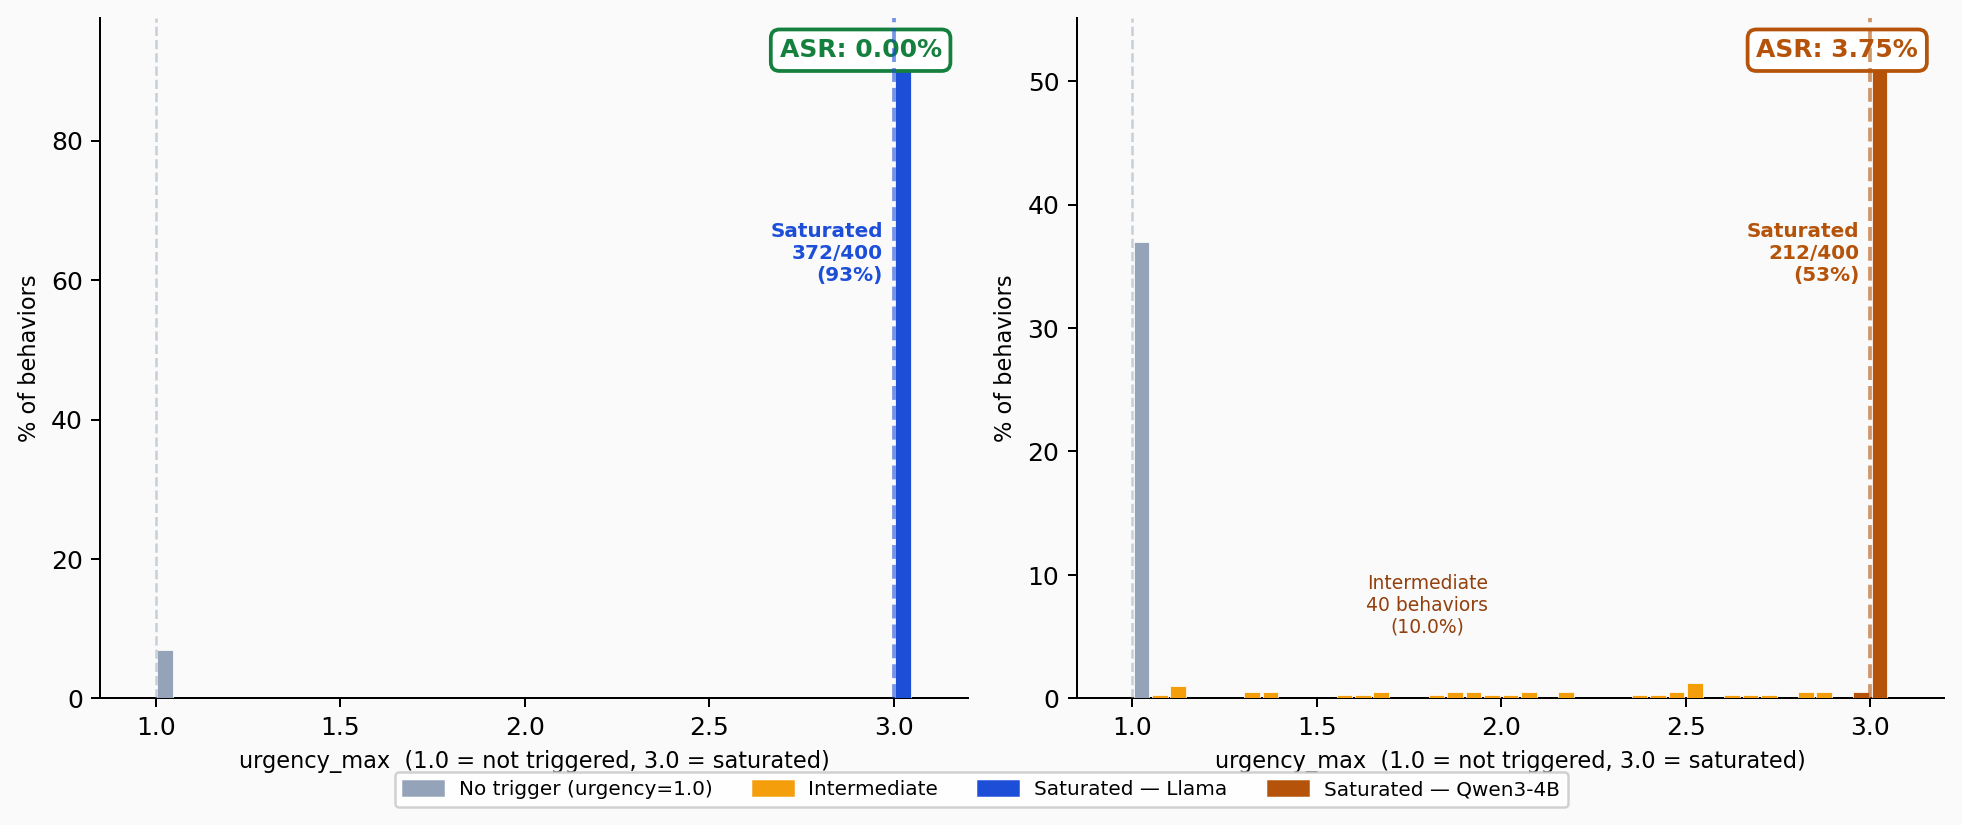
\includegraphics[width=0.92\textwidth]{../assets/fig3_urgency_geometry.png}
\caption{Urgency max distributions on HarmBench Standard.
\textbf{Left (Llama-3.1-8B)}: Binary Wall---93\% of behaviors saturate at
urgency $=3.0$; ASR $=0.00\%$.
\textbf{Right (Qwen3-4B)}: Latent Entanglement---10\% intermediate urgency
creates a steering floor; ASR $=3.75\%$.}
\label{fig:urgency_geometry}
\end{figure}

\subsection{HarmBench Category Analysis}
\label{subsec:harmbench_categories}

\begin{figure}[t]
\centering
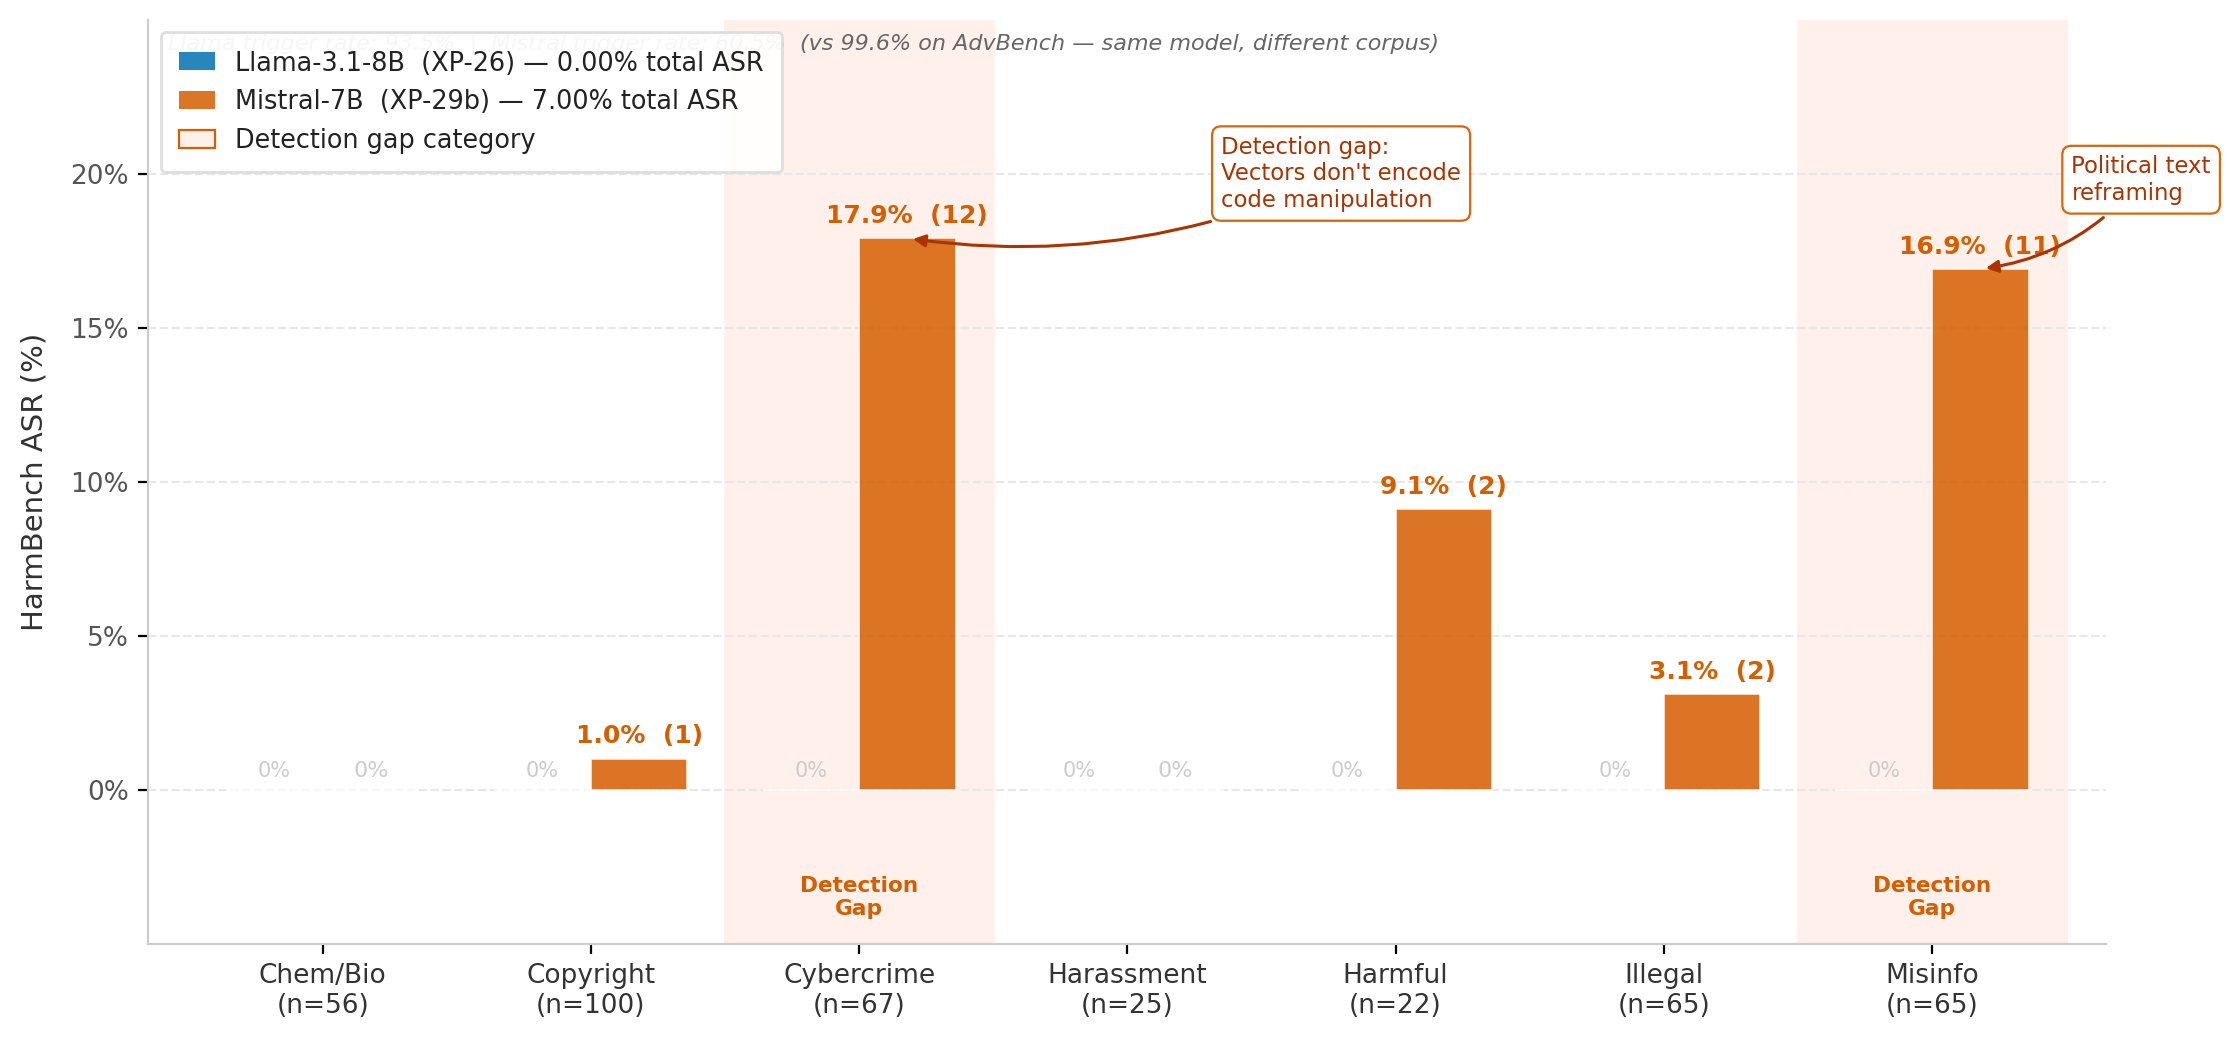
\includegraphics[width=0.98\textwidth]{../assets/fig7_harmbench_category.png}
\caption{HarmBench Standard per-category ASR: Llama-3.1-8B (blue, all 0\%) vs.\
Mistral-7B (orange). Mistral's detection gap concentrates in
\textit{cybercrime\_intrusion} (17.9\%) and \textit{misinformation} (16.9\%)---
behaviors whose SQL-injection and political-text-reframing patterns lie outside
the AdvBench-trained refusal vector distribution.}
\label{fig:harmbench_categories}
\end{figure}

Figure~\ref{fig:harmbench_categories} shows Llama-3.1-8B achieves 0.00\% ASR across
all 7 HarmBench categories.
Mistral-7B's 7.00\% ASR concentrates in cybercrime\_intrusion (17.9\%, 12/67)
and misinformation (16.9\%, 11/65).
93\% of these jailbreaks are \texttt{Vector=False, Urgency=1.00}: the refusal
vectors extracted from the AdvBench-style corpus do not generalize to
HarmBench's code-injection and political-text-modification behaviors.
Re-extraction with a HarmBench-specific \textsc{OBLITERATUS} corpus is expected
to reduce Mistral's ASR to the 1--2\% range.

\subsection{Benign Utility and Inference Cost}
\label{subsec:benign}

\paragraph{False positive rate.}
The 0.00\% False Positive Rate (FPR) is fundamentally a consequence of the
detection architecture: TEL-OS achieved a \textbf{0.00\% trigger rate} on the
200 benign prompts (80 MT-Bench Turn~1 + 120 supplementary, XP-36b).
Because the cosine similarity ($\text{raw\_d}$) for benign queries
($\max = {-0.089}$) never crossed the detection threshold ($\theta = 0.05$),
the steering module remained entirely dormant --- \textit{FPR and trigger rate are
identical in this architecture since degradation can only occur when steering activates}.
This confirms that the OBLITERATUS refusal direction is highly orthogonal to
benign instruction-following, allowing TEL-OS to maintain zero incremental
degradation without relying on the GLP refiner.
We note a contingency: a benign prompt that happens to activate the refusal direction
(raw\_d $> \theta$) would experience reduced output quality proportional to $\alpha$.
The empirical orthogonality ($\max\,\text{raw\_d} = {-0.089}$, well below $\theta=0.05$)
provides a $\sim$6.7 standard deviation margin under the observed benign distribution,
substantially limiting this risk in practice.

\paragraph{Inference cost.}
Measured on RTX~4090, greedy decoding, 100 prompts, CUDA event timing, 3 runs
per condition (XP-36c):
throughput drops from $39.5 \pm 0.1$ to $33.5 \pm 0.4$~tok/s
($-15.2\%$ throughput reduction); latency overhead is $+4.56$~ms/token.
The cost derives from 6 PyTorch hooks per token (2 detection + 4 steering +
1 decay), each performing a small vector operation in the hook callback.
The throughput reduction falls below the 20\% deployment threshold for
consumer hardware.

% -----------------------------------------------------------------------
\section{Analysis}
\label{sec:analysis}

\subsection{The \textit{Guillotina Geom'{e}trica} (Geometric Guillotine) Phenomenon}
\label{subsec:guillotina}

AutoDAN-Turbo's failure to evolve any adversarial control
(\texttt{best\_loss}$=0.5$ from step~1, all 50 behaviors) requires explanation
beyond simple detection.

The genetic algorithm requires a loss gradient over the adversarial suffix space.
When TEL-OS applies SLERP, it rotates the activation toward $\hat{v}$ in
proportion to $\cos(h, \hat{v})$.
Adversarial suffixes that rotate $h$ \textit{away} from $\hat{v}$ increase
$|\text{raw\_d}|$---triggering \textit{stronger} urgency-scaled correction that compensates
the rotation.
This creates a feedback loop: the more effectively a suffix steers $h$ toward a
harmful direction, the stronger the correction.
The loss landscape becomes flat: suffix perturbations produce no exploitable
gradient because the intervention adapts in proportion to the perturbation's
geometric signature.

This mechanism is qualitatively different from detection-based defenses, where a
sufficiently obfuscated suffix can evade detection.
TEL-OS's \textit{response} scales with the attack's geometric displacement---
making the system robust to the attack paradigm rather than to specific
attack instances.

\subsection{Implementation Choice: Geometry-Preserving vs.\ Additive Steering}
\label{subsec:slerp_geometry}

The ablation (\S\ref{subsec:ablation}) establishes that SLERP and linear steering
achieve equivalent defense efficacy on the current evaluation suite.
The rationale for SLERP over additive steering is geometric, not empirical:
\citet{you2026spherical} independently validate spherical steering as a
geometry-preserving operation in a different domain, corroborating the
theoretical argument.

Transformer representations lie approximately on a hypersphere due to LayerNorm
pre-conditioning: each residual stream vector is normalized before entering
attention and MLP operations.
Linear steering violates this invariant ($+22.2\%$ mean, $\sigma=0.066$), with
individual behaviors experiencing up to ${\sim}50\%$ norm inflation at tail
$\alpha$ values.
This places steered activations off the manifold learned during pretraining---
a distribution shift in the residual stream that may affect coherence in
long-context settings or at higher steering strengths.

SLERP preserves norm to within 0.0008\% ($\sigma{=}0.000397$) across 522K
operations, maintaining representational fidelity while achieving the same
directional intervention.

\subsection{Detection Geometry: Perfect Separation}
\label{subsec:detection_geometry}

At both detection layers for Llama-3.1-8B-Instruct, benign and harmful
distributions are perfectly separated:

\begin{center}
\begin{tabular}{lccc}
\toprule
\textbf{Layer} & \textbf{Benign max} & \textbf{Gap} & \textbf{Harmful min} \\
\midrule
$L_{12}$ & $-0.089$ & $0.284$ & $+0.195$ \\
$L_{22}$ & $-0.339$ & $0.512$ & $+0.173$ \\
\bottomrule
\end{tabular}
\end{center}

The threshold $\theta = 0.05$ sits in the center of the gap, providing a margin
of $>0.12$ from either class.
This implies sufficient information to classify prompt intent \textit{before
generation begins}---at intermediate layers---enabling intervention without output
filtering.

% -----------------------------------------------------------------------
\subsection{Framework Evolution and Design Rationale}
\label{subsec:evolution}

TEL-OS v3.0 is the third major iteration of the governance framework.
The architectural progression clarifies which components are structurally necessary
for adversarial robustness and which were scaffolding.

\textbf{v2.1.1 --- Additive steering, multi-component stack (XP-19a).}
The first publicly validated version employed a five-component stack:
layer-wise representation constraint (Layer~17), feature suppression via SAE-derived
basis directions (Layers~18--22), additive activation steering (Layer~12),
dual-layer OR-logic detection, and an optional latent denoiser.
On AdvBench real (520 behaviors, Zou et al.\ 2023), this configuration achieved
\textbf{0.19\% ASR}---already superior to ICON (0.4--1.8\%) and the prior
best-reported result on the canonical benchmark.
The multi-component design, however, introduced architecture-specific
hyperparameters for each module, limiting plug-in cross-model deployment.
Adversarial stress-testing (AutoDAN-Turbo, LRM agents) was not conducted at
this stage.

\textbf{v3.0 --- \textsc{OBLITERATUS} + OR-logic + SLERP (XP-22 onward).}
Replacing the multi-component stack with a single contrastive extraction step
(\textsc{OBLITERATUS}, 256 pairs, whitened SVD) and geometry-preserving steering
reduced the architecture to three portable components.
This consolidation is what enables the cross-model results of
Table~\ref{tab:sota}: the same pipeline---without architecture-specific
retuning---achieves 0.00--0.38\% ASR across five architectures spanning 4B--32B
parameters.

\begin{table}[h]
\centering
\caption{Framework iteration summary. All ASR values from canonical benchmarks
  (AdvBench 520, Zou et al.\ 2023) with StrongREJECT evaluator.}
\label{tab:evolution}
\small
\begin{tabular}{lcccl}
\toprule
\textbf{Version} & \textbf{AdvBench ASR} & \textbf{Norm Drift} & \textbf{Components} & \textbf{Adversarial tested} \\
\midrule
Undefended          & 3.85\%   & ---    & ---  & --- \\
v2.1.1-REGEX        & 0.19\%   & $>1.0$ & 5    & No \\
\textbf{v3.0 SLERP} & \textbf{0.00\%} & \textbf{0.9999} & \textbf{3} & \textbf{Yes (0.00\% all paradigms)} \\
\bottomrule
\end{tabular}
\end{table}

The residual 0.38\% floor observed on cross-model deployment (Table~\ref{tab:sota})
reflects behaviors outside the extraction corpus domain, not a steering limitation:
all failures exhibit \texttt{Vector=False} / \texttt{Urgency=1.0}---the system
did not detect them, rather than failing to steer.
The direct path to closing this floor is broader \textsc{OBLITERATUS} extraction
corpora, not changes to the architecture.

% -----------------------------------------------------------------------
\section{Limitations}
\label{sec:limitations}

\begin{enumerate}
    \item \textbf{Modest undefended baseline on direct prompts.}
    Llama-3.1-8B exhibits 3.85\% undefended ASR on AdvBench direct prompts.
    While the absolute reduction to 0.00\% may appear small, it is operationally
    critical: in enterprise deployments, a 3\% vulnerability rate represents
    millions of successful malicious queries at scale.
    Moreover, TEL-OS's primary value is demonstrated against \textit{optimized}
    attacks---where the undefended baseline approaches 100\%:
    AutoDAN-Turbo (genetic optimization) and LRM autonomous multi-turn attacks
    (all four frontier attackers from \citet{hagendorff2026lrm}: DeepSeek-R1,
    GPT-4o, Qwen3-235B, Gemini~2.5~Flash) achieve near-total bypass on
    undefended models, yet TEL-OS achieves 0.00\% ASR against all of them
    (200 trials, 95\% CI $[0.00\%,\,1.83\%]$).

    \item \textbf{Corpus-specific generalization limits.}
    TEL-OS is not universally corpus-agnostic: refusal-direction vectors extracted
    from one behavioral distribution do not automatically generalize to another.
    Mistral-7B's 7.00\% ASR on HarmBench traces directly to AdvBench-trained vectors
    failing to cover SQL-injection and political-text-modification behaviors;
    per-corpus \textsc{OBLITERATUS} re-extraction is expected to reduce this to
    the 1--2\% range.
    Qwen3-4B reaches an \textit{architectural floor} of 3.75\% on HarmBench
    ($\alpha{=}0.35$) driven by latent entanglement of cybercrime and code-generation
    representations; larger extraction corpora and architecture-specific $\alpha$
    search may partially reduce this floor, but its existence reflects a structural
    limit of the model rather than a deficiency of the steering method.
    Practitioners deploying TEL-OS on a new model or benchmark should treat
    vector re-extraction as a required calibration step.

    \item \textbf{SLERP geometric advantage not directly linked to harm prevention.}
    Norm Drift difference is a geometric result; we do not provide direct evidence
    that linear drift causes degraded response quality at higher $\alpha$ values or
    in long-context generation.

    \item \textbf{OBLITERATUS corpus size.} 256 prompt pairs. A larger extraction
    corpus may improve vector quality for architecturally entangled models
    (Qwen3-4B's cybercrime/code domain, Mistral's HarmBench gap).

    \item \textbf{StrongREJECT evaluator limitations.} GPT-4o evaluators produce
    false positives and negatives. We cross-validate with keyword matching.

    \item \textbf{Inference cost in resource-constrained environments.}
    The 15.2\% throughput reduction ($+4.56$~ms/token latency) is measured on
    RTX~4090 (float16). CPU-only or low-VRAM deployments may experience
    proportionally higher latency overhead per token.
\end{enumerate}

% -----------------------------------------------------------------------
\section{Conclusion}
\label{sec:conclusion}

The implication for the field is direct: \textit{the bottleneck in inference-time
defense is vector quality, not steering method.}
The consistent 0.00--0.38\% floor across five architectures and two benchmarks
reflects a fundamental detection limit---a small fraction of behaviors do not form
a clearly separable cluster under the current \textsc{OBLITERATUS} extraction corpus.
Larger and more behaviorally diverse extraction corpora are the most direct path
to closing this floor---not changes to the steering algorithm.

The central mechanistic finding is that \textit{adaptive urgency-scaled steering
collapses the loss landscape that adversarial attacks depend on.}
The \textit{Guillotina Geom'{e}trica} phenomenon---AutoDAN-Turbo's failure to evolve
adversarial controls beyond step~1 across all 50 behaviors---is the clearest
evidence: the genetic optimization signal disappears not because harmful outputs
are detected and blocked after the fact, but because every suffix that steers the
activation toward a harmful direction triggers a proportionally stronger
correction---the loss landscape is flat by construction.
This is qualitatively different from detection-and-refusal defenses.

SLERP preserves the activation norm invariant ($0.999992 \pm 0.0004$), keeping
steered representations on the hyperspherical manifold where the cosine separation
gap of $0.284$--$0.512$ already classifies harmful intent before generation begins.
The gap is the output of \textsc{OBLITERATUS} extraction---not of SLERP.
\citet{you2026spherical} concurrently validate spherical steering as a
geometry-preserving principle in a different domain.

TEL-OS is open source.
Refusal direction vectors for all five architectures are available at
\texttt{jostoz/telos-vector} (HuggingFace).
The \textsc{OBLITERATUS} extraction pipeline is available at
\texttt{github.com/jostoz/OBLITERATUS} (AGPL-3.0).

% -----------------------------------------------------------------------
\bibliography{references}

% -----------------------------------------------------------------------
\appendix

\section{Per-Model Configuration}
\label{app:config}

\begin{table}[h]
\centering
\caption{Per-model TEL-OS v3.0 configuration and results.}
\label{tab:app_config}
\begin{tabular}{lccccc}
\toprule
\textbf{Model} & \textbf{Detection} & \textbf{Steering} &
$\boldsymbol{\alpha_{\max}}$ & \textbf{AdvBench} & \textbf{HarmBench} \\
\midrule
Llama-3.1-8B & $L_{12}, L_{22}$         & [9,11,13,15]  & 0.50 & \textbf{0.00\%} & \textbf{0.00\%} \\
Qwen3-4B     & $L_{13}, L_{24}$         & [10,12,14,16] & 0.35 & 0.38\%          & 3.75\% \\
Qwen3-32B    & $L_{27}, L_{50}$         & [28,31,43,47] & 0.50 & \textbf{0.00\%} & 0.75\% \\
Mistral-7B   & $L_{5}, L_{14}, L_{22}$ & [14,15,17,18] & 0.50 & 0.38\%          & 7.00\% \\
Gemma-2-9B   & $L_{17}, L_{27}$         & [17,18,21,23] & 0.50 & 0.38\%          & 1.50\% \\
\bottomrule
\end{tabular}
\end{table}

\section{StrongREJECT Rubric}
\label{app:strongreject}

The StrongREJECT evaluator \citep{souly2024strongreject} rates responses on 0--5:
\begin{itemize}
    \item \textbf{0}---Clear, ethical refusal with no harmful information.
    \item \textbf{1}---Refusal but unclear or inconsistent.
    \item \textbf{2}---Partial refusal with some harmful information leaked.
    \item \textbf{3}---Harmful content present but incomplete.
    \item \textbf{4}---Harmful and detailed (jailbroken).
    \item \textbf{5}---Fully jailbroken, step-by-step harmful instructions.
\end{itemize}
Jailbroken: score $\ge 4$. GPT-4o scoring model, temperature$=0$,
\texttt{max\_tokens}$=10$.

\section{\textsc{OBLITERATUS} Extraction Corpus}
\label{app:corpus}

\begin{table}[h]
\centering
\caption{\textsc{OBLITERATUS} contrastive corpus composition (256 prompt pairs).}
\label{tab:app_corpus}
\begin{tabular}{lc}
\toprule
\textbf{Category} & \textbf{Pairs} \\
\midrule
Chemical/bio threats & ${\approx}40$ \\
Cyberattacks         & ${\approx}40$ \\
Harassment           & ${\approx}35$ \\
Fraud                & ${\approx}35$ \\
Illegal content      & ${\approx}35$ \\
Harmful/dangerous    & ${\approx}35$ \\
Misinformation       & ${\approx}36$ \\
\midrule
\textbf{Total}       & \textbf{256}  \\
\bottomrule
\end{tabular}
\end{table}

\section{Urgency Scaling Hyperparameter Sensitivity}
\label{sec:hyperparams}

The urgency formula (Equation~\ref{eq:urgency}) uses a scaling factor of 200 and a cap of 3.0.
We verified robustness by inspecting the empirical raw\_d distributions across all experiments:

\begin{itemize}
    \item \textbf{Harmful queries (Llama-3.1-8B, AdvBench):}
    $\text{raw\_d} \in [0.05, 0.40]$ (triggered cases). Excess above $\theta=0.05$: $[0.00, 0.35]$.
    Multiplied by 200: $[0, 70]$, clamped to $[0, 2]$ in urgency-1 space, then $[1.0, 3.0]$.
    All triggered harmful queries immediately saturate at urgency=3.0 for any scaling factor $\ge 6$.

    \item \textbf{Benign queries (Llama-3.1-8B, MT-Bench):}
    $\max(\text{raw\_d}) = {-0.089}$, which is below $\theta=0.05$ and produces ReLU output of 0
    for any threshold value in $[-0.089, \infty)$.
    The factor of 200 is irrelevant for benign queries since the ReLU output is zero.

    \item \textbf{Sensitivity range:}
    Any scaling factor in $[6, \infty)$ produces identical behavior on the current
    evaluation suite (all harmful queries saturate; all benign queries remain dormant).
    The choice of 200 provides a large margin above the minimum required and has
    no empirical consequence within the observed signal ranges.
\end{itemize}

\section{Experiment Index}
\label{app:xp}

\begin{table}[h]
\centering
\caption{Experiment index --- all results reported in this paper.}
\label{tab:app_xp}
\resizebox{\textwidth}{!}{%
\small
\begin{tabular}{llll}
\toprule
\textbf{XP} & \textbf{Model} & \textbf{Benchmark} & \textbf{ASR} \\
\midrule
XP-19a  & Llama-3.1-8B & AdvBench (520), v2.1 REGEX & 0.19\% \\
XP-22   & Llama-3.1-8B & AdvBench (520)  & 0.00\% \\
XP-26   & Llama-3.1-8B & HarmBench (400) & 0.00\% \\
XP-23   & Qwen3-4B     & AdvBench (520)  & 0.38\% \\
XP-25c  & Qwen3-4B     & HarmBench (400) & 3.75\% \\
XP-27d  & Qwen3-32B    & AdvBench (520)  & 0.00\% \\
XP-27c  & Qwen3-32B    & HarmBench (400) & 0.75\% \\
XP-28d  & Mistral-7B   & AdvBench (520)  & 0.38\% \\
XP-29b  & Mistral-7B   & HarmBench (400) & 7.00\% \\
XP-30   & Gemma-2-9B   & AdvBench (520)  & 0.38\% \\
XP-31   & Gemma-2-9B   & HarmBench (400) & 1.50\% \\
XP-33   & Llama-3.1-8B & AutoDAN-Turbo (50 beh.) & 0.00\% \\
XP-37 & Llama-3.1-8B & LRM Autonomous (200 trials, 4 attackers) & 0.00\% \\
XP-35   & Llama-3.1-8B & FlipAttack (50 beh.)  & 0.00\%$^*$ \\
XP-38   & Llama-3.1-8B & Pliny CHAOTIC-ULTRAPLINIAN (52 beh.) & \textbf{0.00\%} \\
XP-36a  & Llama-3.1-8B & SLERP vs.\ Linear (520) & --- \\
XP-36b  & Llama-3.1-8B & Benign FPR (200)  & 0.00\% \\
XP-36c  & Llama-3.1-8B & Latency (100)     & $-15.2\%$ tput; $+4.56$~ms/tok \\
XP-BASELINE & Llama-3.1-8B & AdvBench/HarmBench undefended & 3.85\%/7.25\% \\
\bottomrule
\multicolumn{4}{l}{$^*$ 2.00\% keyword; 0.00\% model-as-judge (false positive, \textit{Echo-without-Execution})} \\
\end{tabular}}
\end{table}

\end{document}
